\documentclass[a4paper,11pt]{book}
%\documentclass[a4paper,twoside,11pt,titlepage]{book}
\usepackage{listings}
\usepackage[utf8]{inputenc}
\usepackage[spanish]{babel}
\usepackage{graphicx}
\usepackage{url}
\usepackage{eurosym}
\usepackage{listings}
\lstset{basicstyle=\ttfamily, keywordstyle=\rmfamily\bfseries}


% \usepackage[style=list, number=none]{glossary} %
%\usepackage{titlesec}
%\usepackage{pailatino}

\decimalpoint
\usepackage{dcolumn}
\newcolumntype{.}{D{.}{\esperiod}{-1}}
\makeatletter
\addto\shorthandsspanish{\let\esperiod\es@period@code}
\makeatother


%\usepackage[chapter]{algorithm}
\RequirePackage{verbatim}
%\RequirePackage[Glenn]{fncychap}
\usepackage{fancyhdr}
\usepackage{graphicx}
\usepackage{afterpage}

\usepackage{longtable}

\usepackage[pdfborder={000}]{hyperref} %referencia

% ********************************************************************
% Re-usable information
% ********************************************************************
\newcommand{\myTitle}{Diseño e integración de un sistema de clasificación de alteraciones del movimiento de pacientes con rodillas lesionadas: Detección de fatiga basada en entrenamientos de velocidad\xspace}
\newcommand{\myDegree}{Grado en Ingeniería Informática\xspace}
\newcommand{\myName}{Juan Manuel López Castro\xspace}
\newcommand{\myProf}{Oresti Baños Legrán \xspace}
\newcommand{\myOtherProf}{Migel Damas Hermoso\xspace}
%\newcommand{\mySupervisor}{Put name here\xspace}
\newcommand{\myFaculty}{Escuela Técnica Superior de Ingenierías Informática y de
Telecomunicación\xspace}
\newcommand{\myFacultyShort}{E.T.S. de Ingenierías Informática y de
Telecomunicación\xspace}
\newcommand{\myDepartment}{Departamento de ...\xspace}
\newcommand{\myUni}{\protect{Universidad de Granada}\xspace}
\newcommand{\myLocation}{Granada\xspace}
\newcommand{\myTime}{\today\xspace}
\newcommand{\myVersion}{Version 0.1\xspace}


\hypersetup{
pdfauthor = {\myName (email (en) ugr (punto) es)},
pdftitle = {\myTitle},
pdfsubject = {},
pdfkeywords = {palabra_clave1, palabra_clave2, palabra_clave3, ...},
pdfcreator = {LaTeX con el paquete ....},
pdfproducer = {pdflatex}
}

%\hyphenation{}


%\usepackage{doxygen/doxygen}
%\usepackage{pdfpages}
\usepackage{url}
\usepackage{colortbl,longtable}
\usepackage[stable]{footmisc}
%\usepackage{index}

%\makeindex
%\usepackage[style=long, cols=2,border=plain,toc=true,number=none]{glossary}
% \makeglossary

% Definición de comandos que me son tiles:
%\renewcommand{\indexname}{Índice alfabético}
%\renewcommand{\glossaryname}{Glosario}

\pagestyle{fancy}
\fancyhf{}
\fancyhead[LO]{\leftmark}
\fancyhead[RE]{\rightmark}
\fancyhead[RO,LE]{\textbf{\thepage}}
\renewcommand{\chaptermark}[1]{\markboth{\textbf{#1}}{}}
\renewcommand{\sectionmark}[1]{\markright{\textbf{\thesection. #1}}}

\setlength{\headheight}{1.5\headheight}

\newcommand{\HRule}{\rule{\linewidth}{0.5mm}}
%Definimos los tipos teorema, ejemplo y definición podremos usar estos tipos
%simplemente poniendo \begin{teorema} \end{teorema} ...
\newtheorem{teorema}{Teorema}[chapter]
\newtheorem{ejemplo}{Ejemplo}[chapter]
\newtheorem{definicion}{Definición}[chapter]

\definecolor{gray97}{gray}{.97}
\definecolor{gray75}{gray}{.75}
\definecolor{gray45}{gray}{.45}
\definecolor{gray30}{gray}{.94}

\lstset{ frame=Ltb,
     framerule=0.5pt,
     aboveskip=0.5cm,
     framextopmargin=3pt,
     framexbottommargin=3pt,
     framexleftmargin=0.1cm,
     framesep=0pt,
     rulesep=.4pt,
     backgroundcolor=\color{gray97},
     rulesepcolor=\color{black},
     %
     stringstyle=\ttfamily,
     showstringspaces = false,
     basicstyle=\scriptsize\ttfamily,
     commentstyle=\color{gray45},
     keywordstyle=\bfseries,
     %
     numbers=left,
     numbersep=6pt,
     numberstyle=\tiny,
     numberfirstline = false,
     breaklines=true,
   }
 
% minimizar fragmentado de listados
\lstnewenvironment{listing}[1][]
   {\lstset{#1}\pagebreak[0]}{\pagebreak[0]}

\lstdefinestyle{CodigoC}
   {
	basicstyle=\scriptsize,
	frame=single,
	language=C,
	numbers=left
   }
\lstdefinestyle{CodigoC++}
   {
	basicstyle=\small,
	frame=single,
	backgroundcolor=\color{gray30},
	language=C++,
	numbers=left
   }

 
\lstdefinestyle{Consola}
   {basicstyle=\scriptsize\bf\ttfamily,
    backgroundcolor=\color{gray30},
    frame=single,
    numbers=none
   }


\newcommand{\bigrule}{\titlerule[0.5mm]}


%Para conseguir que en las páginas en blanco no ponga cabecerass
\makeatletter
\def\clearpage{%
  \ifvmode
    \ifnum \@dbltopnum =\m@ne
      \ifdim \pagetotal <\topskip
        \hbox{}
      \fi
    \fi
  \fi
  \newpage
  \thispagestyle{empty}
  \write\m@ne{}
  \vbox{}
  \penalty -\@Mi
}
\makeatother

\usepackage{pdfpages}
\begin{document}

\begin{titlepage}
 
\newlength{\centeroffset}
\setlength{\centeroffset}{-0.5\oddsidemargin}
\addtolength{\centeroffset}{0.5\evensidemargin}
\thispagestyle{empty}


\noindent\hspace*{\centeroffset}\begin{minipage}{\textwidth}

\centering

\includegraphics[width=0.9\textwidth]{imagenes/logo_ugr.jpg}\\[1.4cm]

\textsc{ \Large TRABAJO FIN DE GRADO\\[0.2cm]}
\textsc{INGENIERÍA INFORMÁTICA}\\[0.6cm]
% Upper part of the page
% 
% Title
{\Huge\bfseries Diseño e integración de un sistema de clasificación de alteraciones del movimiento de pacientes con rodillas lesionadas\\}
\noindent\rule[-1ex]{\textwidth}{3pt}\\[3.5ex]
%{\large\bfseries Detección de fatiga basada en entrenamientos de velocidad}
\end{minipage}

\vspace{0.9cm}
\noindent\hspace*{\centeroffset}\begin{minipage}{\textwidth}
\centering

\textbf{Autor}\\ Juan Manuel López Castro\\[2.5ex]
\textbf{Directores}\\
{ Oresti Baños Legrán \\
Miguel Damas Hermoso}\\[0.25cm]

\includegraphics[width=0.5\textwidth]{imagenes/etsiit_logo.png}\\[0.25cm]
\textsc{Escuela Técnica Superior de Ingenierías Informática y de Telecomunicación}\\
\textsc{---}\\
%
\includegraphics[width=0.5\textwidth]{imagenes/atc.jpg}\\[0.1cm]
%\textsc{Departamento de Arquitectura y Tecnología de Computadores}\\
%\textsc{---}\\
Granada, Agosto de 2020
\end{minipage}
%\addtolength{\textwidth}{\centeroffset}
%\vspace{\stretch{2}}
\end{titlepage}





\chapter*{}
%\thispagestyle{empty}
%\cleardoublepage

%\thispagestyle{empty}

%\begin{titlepage}
 
 
\setlength{\centeroffset}{-0.5\oddsidemargin}
\addtolength{\centeroffset}{0.5\evensidemargin}
\thispagestyle{empty}

\noindent\hspace*{\centeroffset}\begin{minipage}{\textwidth}

\centering

\includegraphics[width=0.9\textwidth]{imagenes/logo_ugr.jpg}\\[1.4cm]

%\textsc{ \Large PROYECTO FIN DE CARRERA\\[0.2cm]}
%\textsc{ INGENIERÍA EN INFORMÁTICA}\\[1cm]
% Upper part of the page
% 

 \vspace{3.3cm}

%si el proyecto tiene logo poner aquí
%
\includegraphics{imagenes/logo.png} 
 \vspace{0.5cm}

% Title

{\Huge\bfseries Diseño e integración de un sistema de clasificación de alteraciones del movimiento de pacientes con rodillas lesionadas\\
}
\noindent\rule[-1ex]{\textwidth}{3pt}\\[3.5ex]
{\large\bfseries  Detección de fatiga basado en entrenamientos de velocidad\\[4cm]}
\end{minipage}

\vspace{2.5cm}
\noindent\hspace*{\centeroffset}\begin{minipage}{\textwidth}
\centering

\textbf{Autor}\\ {Juan Manuel López Castro}\\[2.5ex]
\textbf{Directores}\\
{Oresti Baños Legrán \\
Miguel Damas Hermoso}\\[2cm]

%\includemovie{3cm}{3cm}{imagenes/tstc.gif}

\includegraphics[width=0.5\textwidth]{imagenes/atc.jpg}\\[0.1cm]
\textsc{Departamento de Arquitectura y Tecnología de Computadores}\\
\textsc{---}\\
Granada, Agosto de 2020
\end{minipage}
\addtolength{\textwidth}{\centeroffset}
\vspace{\stretch{2}}

 
\end{titlepage}






\cleardoublepage
\thispagestyle{empty}

\begin{center}
{\large\bfseries  Diseño e integración de un sistema de clasificación de alteraciones del movimiento de pacientes con rodillas lesionadas}\\
\end{center}
\begin{center}
Juan Manuel López Castro\\
\end{center}

%\vspace{0.7cm}
\noindent{\textbf{Palabras clave}: EMGs, fatiga, clasificación, lesión, diagnóstico, LCA, sistema nervioso central, aprendizaje automático, selección de características  }\\

\vspace{0.7cm}
\noindent{\textbf{Resumen}}\\

En la actualidad la electromiografía de superficie está jugando un papel muy importante apoyando a los fisioterapeutas y médicos para analizar el rendimiento de atletas y pacientes, así como para detectar posibles problemas musculares a la hora de realizar tanto una actividad física como una actividad cotidiana. 

Existen evidencias de que personas con lesiones en la rodilla, como por ejemplo, la rotura total o parcial del ligamento anterior cruzado, sufren cierta compensación muscular entre el cuadriceps y el isquiotibial. Basándonos en esto se plantea realizar un sistema automático para la detección de la fatiga muscular. Con dicho sistema un fisioterapeuta podría hallar que músculos entran en fatiga antes y determinar si hay o no cierta compensación entre músculos antagonistas, y por lo tanto probabilidad de mal funcionamiento de la rodilla debido a una lesión. 

Para ello se ha realizado un estudio sobre que tipos de clasificadores obtienen un mejor rendimiento a la hora de clasificar las señales de electromiografía entre fatiga y no fatiga. Se han hecho uso de datos de electromiografía tomados a un conjunto de bomberos que han realizado sentadillas, todos con un peso cargado del 70 por ciento de su RM. En cada repetición tomada también se ha registrado la velocidad de ejecución, para poder estimar la fatiga muscular.

\cleardoublepage


\thispagestyle{empty}


\begin{center}
{\large\bfseries Design and integration of a classification system for movement disorders in patients with injured knees}\\
\end{center}
\begin{center}
Juan Manuel López Castro\\
\end{center}

%\vspace{0.7cm}
\noindent{\textbf{Key words}: EMGs, fatigue, detection, injury, medical diagnostic, Central Nervous System, machine learning, feature selection  }\\

\vspace{0.7cm}
\noindent{\textbf{Abstract}}\\

Nowadays surface electromyography is playing a important role supporting to physiotherapist and medics to analyse athlete's performance as well as to detect possible muscular problems when they are performing some activity.

There is evidence that people with knee injuries, such as a total or partial tear of the anterior cruciate ligament, suffer some muscle compensation between the quadriceps and the hamstring. Based on this, the goal is create an automatic system for the detection of muscle fatigue. With this system, a physiotherapist could find that muscles go into fatigue earlier and determine whether or not there is some compensation between antagonist muscles and therefore the probability of knee malfunction due to injury.

To solve the problem, a study about which types of classifiers have better performance when classifying electromyography signals between fatigue and non-fatigue. Electromyography data was taken from a set of firefighters who have performed squats, all with a loaded weight of 70 percent of their MR. In each repetition taken, the execution speed has also been recorded, to be able to estimate muscle fatigue.





\chapter*{}
\thispagestyle{empty}

\noindent\rule[-1ex]{\textwidth}{2pt}\\[4.5ex]

Yo, \textbf{Juan Manuel López Castro}, alumno de la titulación INGENIERÍA INFORMÁTICA de la \textbf{Escuela Técnica Superior
de Ingenierías Informática y de Telecomunicación de la Universidad de Granada}, con DNI 77023144P, autorizo la
ubicación de la siguiente copia de mi Trabajo Fin de Grado en la biblioteca del centro para que pueda ser
consultada por las personas que lo deseen.

\vspace{6cm}

\noindent Fdo: Juan Manuel López Castro

\vspace{2cm}

\begin{flushright}
Granada a 2 de Septiembre de 2020
\end{flushright}


\chapter*{}
\thispagestyle{empty}

\noindent\rule[-1ex]{\textwidth}{2pt}\\[4.5ex]

D. \textbf{Oresti Baños Legrán }, Profesor del Área de Ingeniería de Sistemas y Automática del Departamento de Arquitectura y Tecnología de Computadores de la Universidad de Granada.

\vspace{0.3cm}

D. \textbf{Miguel Damas Hermoso}, Profesor del Área de Arquitectura y Tecnología de Computadores del Departamento de Arquitectura y Tecnología de Computadores de la Universidad de Granada.


\vspace{0.3cm}

\textbf{Informan:}

\vspace{0.3cm}

Que el presente trabajo, titulado \textit{\textbf{Diseño e integración de un sistema de clasificación de alteraciones del movimiento de pacientes con rodillas lesionadas}},
ha sido realizado bajo su supervisión por \textbf{Juan Manuel López Castro}, y autorizamos la defensa de dicho trabajo ante el tribunal
que corresponda.

\vspace{0.3cm}

Y para que conste, expiden y firman el presente informe en Granada a 2 de Septiembre de 2020

\vspace{0.3cm}

\textbf{Los directores:}

\vspace{5cm}

\noindent \textbf{Oresti Baños Legrán \ \ \ \ \ Miguel Damas Hermoso}

\chapter*{Agradecimientos}
\thispagestyle{empty}

       \vspace{1cm}


Gracias por el apoyo a todos mis familiares y amigos.


\frontmatter
\tableofcontents
\listoffigures
\listoftables

\mainmatter
\setlength{\parskip}{5pt}


\chapter{ Introducción}
Breve introducción donde se explica la motivación de dicho trabajo, como ha sido planteado en el tiempo, sus objetivos principales y secundarios y la estructura que tiene cada uno de los capítulos que forman la memoria.
\section{Motivación}
Cierto es que el uso de la informática y la tecnología está en auge en nuestra sociedad. Esto está llegando no solo a facilitar nuestra vida cotidiana, sino también a apoyar y beneficiar la aplicación de la medicina y la salud. Por ejemplo, la electromiografía (EMG) es de gran utilidad para analizar el comportamiento y la activación de las unidades motoras (Figura \ref{fig:motoneurona}) a la hora de realizar cierta actividad física. Esto, junto con la multitud de características que se pueden extraer de las señales EMG adquiridas, hace que se puedan realizar multitud de estudios para analizar el rendimiento y patologías de pacientes. Haciendo uso de un buen diseño e implementación se puede llegar a obtener un sistema de tiempo real donde se pueda realizar el diagnostico en el mismo momento de la actividad física y poder analizar los diferentes datos tomados \cite{konrad2005abc}.

\begin{figure}[ht]
\centering
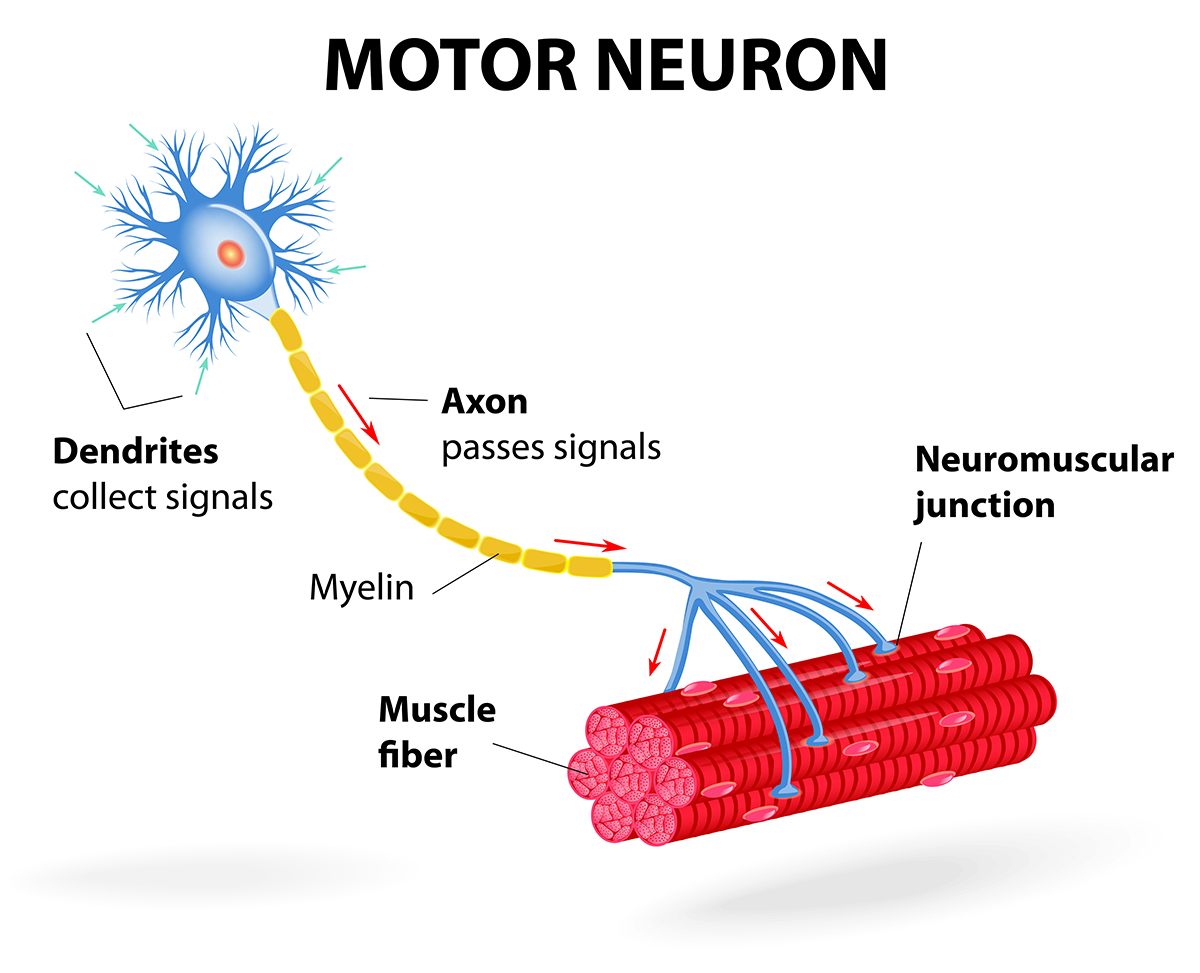
\includegraphics[scale=0.25]{imagenes/motoneurona.jpg}
\vspace{-1.0cm}
\caption{ Ejemplo de motoneurona \cite{motoneurona1}}
\label{fig:motoneurona}
\end{figure}
Existe un gran número de deportistas que cuando entrenan hacen todo lo posible para evitar la fatiga muscular. Por ejemplo, sería el caso de atletas que practican powerlifting o halterofilia, donde el objetivo es levantar el mayor peso posible en una sola repetición. Estos atletas evitan los entrenamientos bajo fatiga debido a que cuando entrenan bajo fatiga no consiguen un rendimiento óptimo. Esto se debe a que cuando se entrena bajo fatiga, el esfuerzo que se tiene que realizar es mucho mayor, así como la probabilidad de lesión. Además aunque el esfuerzo realizado sea mayor, no implica que la fuerza ejercida sobre la carga levantada también lo sea, ya que no se están reclutando tantas fibras musculares.

El aumento del esfuerzo realizado y la mayor probabilidad de lesión se deben a que cuando el sistema nervioso central entra en fatiga no recluta tantas unidades motoras y por ende, no existe tanta activación muscular. Como sabemos la musculatura complementa al sistema óseo y por lo tanto un déficit en la implicación de algún músculo debido a la fatiga hará que se incremente la posibilidad de lesión en articulaciones y ligamentos. Por ejemplo, en algunas lesiones de rodilla como la rotura del ligamento cruzado anterior, se produce una compensación entre cuádriceps e isquiotibial. Una entrada en fatiga de ambos músculos, quitaría mucha estabilidad a la rodilla y aumentaría el daño en el ligamento. Si el ligamento, en lugar de sufrir una rotura total, solo estuviese roto parcialmente, es decir, una lesión más leve, lo que se conseguiría entrenando bajo fatiga sería incrementar la lesión.
Todo esto se explica con mayor detalle en el capítulo \ref{analisis} .

En este proyecto se ha tratado de desarrollar una herramienta que ayuda a los fisioterapeutas a la hora de detectar la fatiga muscular. Con ello se pretende dotar al fisioterapeuta de la suficiente información como para determinar que músculo ha experimentado dicha fatiga y así poder estudiar si se ha producido una compensación muscular a la hora de la ejecución de una sentadilla y determinar si hay una lesión en dicha rodilla. Además, como se ha comentado en párrafos anteriores, en multitud de sistemas de entrenamientos basados en fuerza, está desaconsejado el entreno bajo fatiga, ya que se considera contraproducente. Esto implica otro posible uso de dicho sistema, y es que podría ser utilizado por atletas expertos, en entrenamientos de fuerza como powerlifting o halterofilia para detectar la fatiga en el momento del entreno y cortar la serie para descansar y no tener un entreno contraproducente. 

Para determinar la fatiga en este proyecto, se ha puesto la condición de que cuando un atleta está realizando una serie de sentadillas y su velocidad de ejecución decae un 20 por ciento, es un indicativo de fatiga. Esta condición se debe de cumplir en dos repeticiones seguidas, para así determinar una fatiga más representativa. La condición de la caída de velocidad fue propuesta por el fisioterapeuta de la empresa encargada de la toma de datos, mDurance \cite{mDurance}, además de ser bastante utilizada en el mundo del deporte \cite{fernandezpropuesta}.

Cabe destacar que este proyecto ha sido llevado a cabo con la colaboración de mDurance \cite{mDurance}, una empresa especializada en electromiografía y que ha sido la encargada de aportar los datos para realizar el estudio de los diferentes clasificadores. Han aportado datos de electromiografía sobre los músculos vasto medial y recto femoral de ambas extremidades inferiores a la hora de realizar sentadillas.


\section{Planteamiento del trabajo}
Para solucionar el problema de la detección de la fatiga muscular y también poder determinar si existe o no compensación muscular y por ende una lesión en la rodilla se pretende desarrollar un modelo que clasifique las señales de EMG recibidas entre fatiga y no fatiga. 

Para ello, el desarrollo del modelo consta de tres fases principales. Una primera fase de extracción de características de la señal EMG, tales como RMS, MAV, MDF, etc. En el capítulo \ref{cap6} se comentan todas las características estudiadas junto con su definición. Una segunda fase de selección de las características más representativas de la fatiga, para quedarnos con la menor cantidad posible y así obtener un clasificador más eficiente y rápido. Finalmente una fase de clasificación donde se probarán diferentes clasificadores para finalmente quedarnos con el que mejor prestaciones tenga para dicho problema. 
Con dicho clasificador se podría clasificar las señales EMG recibidas en tiempo real para determinar si la persona que está realizando las repeticiones de sentadillas ha sufrido fatiga y en el momento en el que la ha sufrido. 

Con esta herramienta los fisioterapeutas y médicos podrían realizar pruebas a sus pacientes para luego llegar a ciertas conclusiones. Todo esto sin la necesidad de tener una maquinaria muy compleja, ya que una vez implementado y entrenado el clasificador, no sería necesario medir la velocidad de ejecución de las series de los pacientes a los que se va a realizar la prueba.

Por último comentar que para la realización de este proyecto han sido necesarios datos reales, tomados y filtrados por la empresa especializada en electromiografía mDurance. Además de los datos de las diferentes señales de electromiografía, fue necesario una medición de la velocidad de cada repetición para así, al tener la velocidad de cada repetición poder estimar que sujetos experimentaron fatiga y utilizar dichos datos para entrenar y analizar el rendimiento de los diferentes clasificadores.
\section{Objetivos\label{objetivos}}

Como consecuencia de lo planteado anteriormente el objetivo general sería obtener un clasificador que reciba los datos de la señal EMG y clasifique en tiempo real entre fatiga y no fatiga. Esto servirá para detectar la fatiga en tiempo de ejecución con una herramienta muy sencilla y una vez entrenado el modelo, no sería necesario la utilización de un velocímetro para medir la velocidad de ejecución de cada repetición y estimar la fatiga. Esto se debe a que nuestro modelo, una vez entrenado, solo por el análisis de las señales será capaz de catalogar las señales de EMG entre fatiga y no fatiga. Además una vez clasificadas las señales EMG, el personal especializado para ello podrá determinar si existe compensación entre músculos implicados en el movimiento normal de la rodilla y determinar si existe algún tipo de lesión.

Con respecto a los objetivos específicos, están muy relacionados con las tres fases comentadas anteriormente.
\begin{itemize}
\item Analizar y procesar las señales brutas de EMG.
\item Analizar la velocidad registrada de cada sujeto.
\item Estimar la fatiga de cada uno de los sujetos.
\item Extraer características de las señales de EMG.
\item Crear los archivos de entrenamiento-testeo.
\item Seleccionar las características más útiles para el modelo final.
\item Clasificar las señales de EMG. 
\item Validar el rendimiento de los modelos.
\end{itemize}
\section{Estructura del trabajo}
En este capítulo 1, todo lo comentado es una breve introducción al problema a resolver y a la realización del proyecto. Más adelante se explicarán con más detalle las pautas que se han seguido para el desarrollo del proyecto.

En el capítulo 2 se comenta el estado del arte donde se hará un análisis en profundidad del problema en cuestión, de toda la tecnología que abarca y su posible aplicación en la actualidad.


En el capítulo 3 se comenta la planificación llevada a cabo para la realización del proyecto, así como el coste económico final y parcial.

En el capítulo 4 se hace un análisis del problema tratado. La fatiga muscular, como afecta al sistema nervioso y los problemas musculares asociados a las lesiones de rodilla.

En el capítulo 5 se realiza un diseño de todas las fases realizadas para el proyecto. Consta de un gran número de esquemas donde se explica el funcionamiento de los algoritmos utilizados y los tipos de archivos de entrenamiento-testeo implementados.

El capítulo 6 es el dedicado a la implementación. En él se puede encontrar el código asociado al desarrollo del proyecto.

El capitulo 7 está dedicado a la sección de pruebas. En él se pueden encontrar todos los resultados de los clasificadores diseñados y una opinión personal sobre sus rendimientos.

Por último, el capítulo 8 es el dedicado a las conclusiones y trabajos futuros. En él se comenta si se han cumplido los objetivos de este proyecto y consejos para una futura aplicación junto a una herramienta de electromiografía.




\chapter{Estado del arte}
A continuación se explica a fondo la temática de este proyecto, así como sus posibles aplicaciones en la actualidad. 

\section{EMG}
La electromiografía se ha convertido en una de las técnicas más utilizadas en la actualidad para estudiar el potencial de acción de los músculos. Hacen uso de ella tanto neurofisiólogos, neurólogos y rehabilitadores. Se basa en la captación de las señales electromiográficas, las cuáles, son señales producidas por la musculatura a la hora de realizar una fase de contracción o relajación. Esta fase de contracción o relajación es producida por el estímulo de las motoneuronas. Existen dos tipos de motoneuronas. En este ámbito nos referimos a las motoneuronas somáticas que son las encargadas de las contracciones y relajaciones de la musculatura cuya acción es voluntaria.

Las motoneuronas forman parte de las unidades motoras (Figura \ref{fig:unidad motora}). Una unidad motora es realmente la encargada de las contracciones y relajaciones musculares y está formada por el conjunto de fibras musculares que afecta y la motoneurona encargada de enviar el estímulo. Cuando el impulso eléctrico de la motoneurona llega a las fibras musculares que afecta se obtiene un potencial de activación. El conjunto de todos los potenciales de activación de todas las fibras musculares que son activadas por una motoneurona se le conoce como el potencial de acción de la unidad motora. Lo que se analiza en la electromiografía es la actividad de las múltiples unidades motoras encargadas de un músculo \cite{konrad2005abc,suarez2013bases}.

\begin{figure}[ht]
\centering
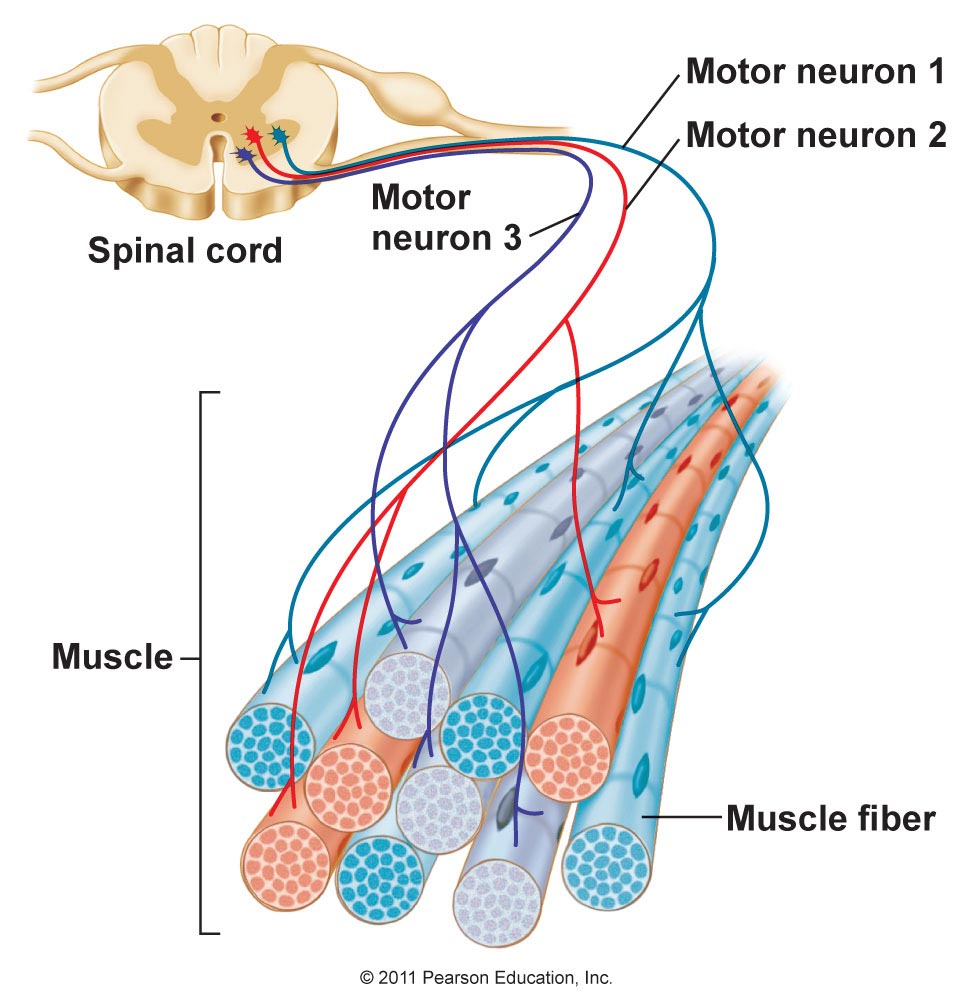
\includegraphics[scale=0.4]{imagenes/unidad motora.jpg}
\caption{Ejemplo de unidad motora \cite{unidadmotora}}
\label{fig:unidad motora}
\end{figure}

Estos impulsos eléctricos generados por las motoneuronas somáticas y que contraen o relajan el músculo son registrados en forma de señales electromiográficas y son utilizadas para ayudar a diagnosticar problemas de salud, que a simple vista, no pueden ser identificados. 

Para medir estas señales electromiográficas se pueden seguir dos métodos, el superficial y el intramuscular \cite{konrad2005abc}.

En la electromiografía intramuscular (Figura \ref{fig:intramuscular}), se utiliza una aguja electrodo para medir la actividad muscular. Esta aguja es introducida por la piel hasta llegar al músculo que queremos estudiar. Es mucho más precisa que la electromiografía de superficie, ya que al ser una aguja introducida directamente en el músculo, no recibe ruido externo de músculos adyacentes al estudiado. Por el contrario es más incomoda, ya que cada vez que se quiera hacer dicho análisis el paciente debe de ser pinchado, y puede que no esté dispuesto a dicho tratamiento. Además si se quiere analizar un actividad física compleja, como salto vertical, horizontal, carrera o sentadilla, como en el caso de este proyecto, el tener unas agujas introducidas en la musculatura puede ser molesto y hacer que la actividad física no se desarrolle a plenitud. Por último, para la utilización de esta técnica, se deberían de tener ciertos conocimientos médicos, ya que una persona sin dichos conocimientos no puede ser capaz de realizar el análisis de la forma correcta, al no conocer por ejemplo, el lugar óptimo para introducir la aguja. Otro agravante es que sin estos conocimientos, se podría llegar hasta la lesión del paciente, debido a introducir la aguja en el lugar no indicado. 

En la electromiografía de superficie (Figura \ref{fig:superficial}) se utilizan electrodos situados en la piel, que captan dichas señales electromiográficas. Es un método no invasivo y fácil de utilizar, donde solo es necesario tener el conocimiento de cual es el lugar óptimo para la colocación de los electrodos. Existen varios tipos de electrodos que serán explicados en el próximo apartado. En este proyecto se ha hecho uso de la electromiografía de superficie.


\begin{figure}[!ht]
\centering
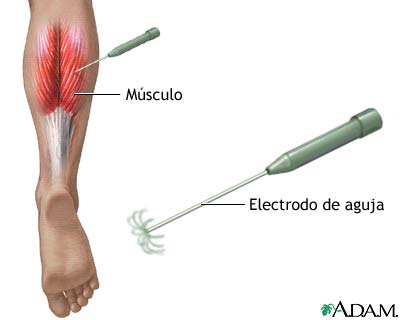
\includegraphics[scale=0.4]{imagenes/electrodo intramuscular.jpg}
\caption{Electromiografía intramuscular \cite{electrodoIntramuscular}}
\label{fig:intramuscular}
\end{figure}


\begin{figure}[!ht]
\centering
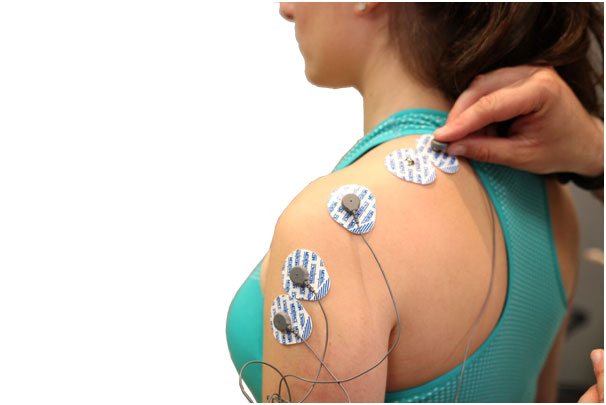
\includegraphics[scale=0.4]{imagenes/electrodo de superficie.jpg}
\caption{Electromiografía de superficie \cite{electrodoSuperficial}}
\label{fig:superficial}
\end{figure}



\subsubsection{EMG de superficie}
Para la realización de este proyecto se ha hecho uso de la electromiografía de superficie (EMGs). Esta técnica implica la utilización de electrodos situados en la piel, para la captación de las señales eléctricas. Por esto mismo, es necesario que en la mayoría de las ocasiones, para una mayor precisión en los datos tomados se realice una preparación de la piel en donde se van a situar los electrodos.

Por ejemplo, para que los electrodos queden mejor adheridos a la piel, a veces es necesario rasurar la piel para eliminar los pelos y que haya más superficie de contacto. También suele ser necesario limpiar la piel para eliminar partículas que dificulten la adherencia de los electrodos. Existen también electrodos que necesitan de la aplicación de un gel para su colocación, para así aumentar la precisión del electrodo. La funcionalidad de este gel es aumentar la conductividad entre la piel y el electrodo.

Otro factor importante es el tamaño del electrodo. Cuanto más pequeño sea, más precisión muscular nos dará, ya que, no cubrirá tanta superficie y no captará así actividad de músculos en los que no estamos interesados. El tamaño de los electrodos debería ser de 1 cm o menor \cite{konrad2005abc}.
\section{Aplicaciones médicas}
Como se ha comentado en secciones anteriores, el estudio de las señales de electromiografía es de gran utilidad para diagnosticar problemas motores y de salud. Algunas de estas enfermedades son: \cite{luzar2005electromiografia}
\begin{itemize}
\item Enfermedad de la neurona motora, ELA.
\item Radioculopatías, afectan a la columna vertebral, como por ejemplo, la ciática o la hernia de disco.
\item Plexopatías. Es difícil de conocer su origen. Produce un dolor y falta de movilidad en el brazo u hombro. Con el uso de la EMG intramuscular se puede llegar a conocer su origen.
\item Mononeuropatías agudas. Implican un daño en la medula espinal y produce hormigueo en la zona afectada.
\item Miopatía. Anomalía o mal funcionamiento en un grupo muscular, debido a un mal impulso eléctrico de las neuronas o a un mal funcionamiento del grupo muscular.
\end{itemize}

En este último punto va a ir centrado el proyecto, en facilitar el diagnostico de rodillas lesionadas a los fisioterapeutas que hagan uso de dicha herramienta. Para ello hace falta indagar en la base de la fatiga muscular y en que se ha basado el proyecto.

\section{Entrenamientos basados en velocidad y fatiga}
En la actualidad existe gran interés entre los atletas tanto profesionales como no profesionales, de mejorar su rendimiento. Para ello es indispensable pensar en un buen entrenamiento, ya que es la base de un buen rendimiento en la competición final. Para ello diversos estudios se han centrado en detectar la fatiga en los entrenamientos, ya que se considera, que entrenar bajo fatiga lo único que nos aporta es un lastre en el entrenamiento, ya que no reclutamos todas la unidades motoras necesarias y no se estimula lo suficiente al músculo. Además de que esto también supone un daño muy alto al sistema nervioso central.

Uno de los factores que indica la fatiga es la perdida de velocidad de ejecución en las actividades físicas, como por ejemplo, en las sentadillas. Se considera que una perdida del 20 por ciento en la velocidad de ejecución es indicativo de que existe una fatiga y por lo tanto se debe proceder a cortar la serie de entrenamiento y dar unos minutos de descanso para proseguir cuando el sujeto ya no esté sufriendo dicha fatiga \cite{fernandezpropuesta}.

Esta técnica dota al atleta de una gran capacidad de entrenamiento, ya que de dicha manera entrenará sin llegar a su limite y realizando siempre series efectivas, las cuáles, harán que se reclute el mayor número de unidades motoras y así obtener una mayor fuerza y desarrollo muscular. 

\section{Aplicación a este proyecto}

Como se ha explicado la electromiografía ha permitido grandes avances en la medicina y en el mundo del deporte. Este proyecto está más encaminado hacia los fisioterapeutas. Pretende desarrollar un sistema de clasificación, para que, sin la necesidad de medir la velocidad de ejecución de las series, se pueda determinar en el momento exacto de la prueba si el atleta está experimentando o no fatiga. Esto será de gran utilidad a atletas que quieran mejorar sus entrenamientos, así como, para que los fisioterapeutas obtengan más información, complementaria a los valores utilizados para la determinación de la actividad muscular como RMS, MNF, MDF, MAV, etc. 

Con toda esta información podrían llegar a conclusiones muy interesantes, tales como, en la ejecución de una sentadilla ver que músculos son los que entran en fatiga y determinar si se está produciendo una compensación muscular debido a una lesión de rodilla o por ejemplo, si dicho músculo está sufriendo algún tipo de daño y por ende su bajo rendimiento y fatiga tan temprana.
También puede ser utilizada para mejorar el rendimiento a la hora de entrenar, ya que detectaría la fatiga en tiempo real, y dotaría al atleta de una información real sobre su fatiga y así podría determinar si se necesita un descanso o por el contrario seguir realizando la actividad física.


%\chapter{Especificación de requisitos}
En este capítulo se tratarán tanto los requisitos funciones como los no funcionales del proyecto. Con esto se obtendrá una idea general sobre la funcionalidad final que se quiere obtener.

\section{Requisitos funcionales}
Como bien es sabido, los requisitos funcionales definen la funcionalidad de nuestro sistema software. Los requisitos funcionales de este proyecto son:
\begin{itemize}
\item Captar las señales de electromiografía durante la actividad física en cuestión, en este caso, sentadillas.
\item Filtrar las señales obtenidas con el fin de obtener el menor ruido posible.
\item Analizar la activación muscular de cada señal, para determinar el tamaño de ventana de cada repetición.
\item Obtener las características más representativas de la señal.
\item Analizar la velocidad registrada y asignar a cada repetición la correspondiente fatiga.
\item Seleccionar las características más representativas de la fatiga.
\item Crear un dataset con las características para la clasificación.
\item Normalizar el dataset de las características, para así aumentar el rendimiento del software.
\item Clasificación de las señales entre fatiga y no fatiga.
\item Aviso visual y sonoro en caso de detectar dicha fatiga.


\end{itemize}

\section{Requisitos no funcionales}
Con respecto a los requisitos no funcionales, son los encargados de dictar las condiciones básicas que debe de seguir nuestro software, es decir, las características generales. Los requisitos no funcionales serían los siguientes:
\begin{itemize}
\item Sistema intuitivo de usar y cómodo a la hora de llevar puesto para la realización de la actividad física.
\item Conexión a dispositivo Android que muestre los resultados en tiempo real.
\item Rendimiento óptimo, para si obtener la menor latencia posible.
\item Buen electromiógrafo, para un mayor rendimiento.
\end{itemize} %diferentes tipos de dataset 

\chapter{Planificación y coste}
Este capítulo trata sobre la planificación llevada a cabo y el coste total de la implementación. Con respecto a la planificación se explica tanto la planificación llevada con los tutores responsables de dicho proyecto como la planificación personal a la hora de desarrollar el proyecto.

\section{Planificación}
La planificación de este proyecto comenzó con una reunión a finales de noviembre de 2019, para tratar el problema a resolver. La reunión fue llevada a cabo por Miguel Damas Hermoso, Oresti Baños Legrán, ambos tutores de este proyecto e Ignacio Díaz Reyes, CEO de mDurance, empresa encargada de aportar todas las herramientas necesarias para la toma de datos, así como, los datos en cuestión para la realización de este proyecto.
En esta reunión se debatió sobre la temática del proyecto y sobre lo que se intentaba aportar con dicha solución. También se comentó el "dataset" que iba a ser utilizado para el estudio, el cuál se iba a encargar de tomar un centro de Barcelona que trabajaba junto a mDurance.

Para finalizar se me realizó una prueba con la herramienta que iba a ser utilizada para medir las señales de electromiografía para ver como funcionaba y aumentar mi conocimiento sobre el tema.

A continuación se explica el restante de las reuniones llevadas a cabo y la planificación personal a la hora de desarrollar el proyecto.

\subsection{Sesiones formativas y reuniones}

Con respecto a la adquisición de conocimientos sobre electromiografía, toma de datos, filtración y amplificación de las señales tomadas, recibí dos sesiones formativas en el centro de mDurance de aproximadamente dos horas. En estas reuniones Ignacio Díaz Reyes realizó una introducción hacia la electromiografía y de sus aplicaciones en el mundo actual. A parte de esto, también nos habló sobre las diferentes características de las señales, sobre todo de las más conocidas y utilizadas en la actualidad.
Esto fue complementado mostrando análisis realizados sobre pacientes para ver como se puede diagnosticar ciertos déficits en la musculatura solo con extraer características de las señales EMG. Por último comentar que me facilitó documentación sobre la EMG y sobre sus características, tanto en el dominio del tiempo como en el dominio de la frecuencia.

Después de estas dos sesiones, que se realizaron el 21 de enero y el 11 de febrero de 2020, ya estaba preparado para empezar el proyecto en la fase de extracción de características de la señal EMG.

La próxima reunión que realizamos fue por medio de GoogleMet, ya que había un problema con los datos que supuestamente iban a ser utilizados para el proyecto. Debido al COVID-19 y a la declaración del estado de alarma, dichos datos no pudieron ser tomados, por lo que nos encontrábamos a mitad de marzo y sin datos para poder realizar el proyecto. Esta reunión fue clave para poder realizar el proyecto. En ella, ambos tutores, junto con Ignacio y Carlos, el fisioterapeuta de mDurance, hicimos una puesta en común de ideas para poder obtener otro "dataset" que supliera al original. Se acordó realizar una búsqueda sobre posibles ideas y zanjar el problema en una próxima reunión.

En la siguiente reunión, unos tres días posterior a la anterior, Ignacio aportó una solución, ya que había hablado con un colaborador que se iba a encargar de tomar un nuevo "dataset". Esta nueva orientación era muy parecida a la original, solo que añadía una nueva idea, la fatiga. Con esto además de hallar que pacientes sufrían de rodilla lesionada, también podía ser utilizado para detectar la fatiga muscular. Este "dataset" trataba sobre un ejercicio multiarticular, la sentadilla. Se acordó que dispondría de los datos en la mayor brevedad posible. Finalmente tuve acceso a parte de los datos el 24 de mayo y el 20 de junio a la totalidad de ellos. Por lo que esto implicó la imposibilidad de poder presentar el proyecto en la primera convocatoria.

Una vez que ya disponía de los datos, a partir del 13 de julio, tuve reuniones consecutivas con ambos tutores, para ir mostrándoles como iba el desarrollo del proyecto e ir acordando el formato de la memoria y todo lo que debía de añadir.

El 27 de julio tuvimos una ultima reunión donde les mostré un prototipo bastante avanzado del desarrollo, el cual, vieron bastante bien, y se acordó que ya solo tenía que desarrollar el proyecto final y complejo, así como el desarrollo de la memoria. 

Para la memoria se acordó enviar un prototipo para mediados de agosto, y la memoria final para el 3 de septiembre, para así tener siempre un margen de error y poder corregir posibles errores antes de la entrega final de los proyectos.

Con respecto a mi propio trabajo, se comenta en la siguiente sección. 

\subsection{Implementación y memoria}

Una vez realizadas las dos sesiones formativas de EMG comentadas anteriormente, ya podía empezar a indagar en el tema de la electromiografía y su análisis de datos. Durante los meses de enero, febrero y marzo, debido a la incertidumbre de los datos explicada, tuve acceso a unas señales EMG de prueba facilitadas por mDurance para poder hacer el desarrollo de la extracción de las características. Durante estos meses fui obteniendo más conocimientos sobre las señales de EMG, sus características y utilidad, así como, sobre la clasificación binaria de dichas señales. Además con los datos de prueba, pude realizar la implementación de los algoritmos de extracción de características que yo consideré más relevantes para la realización de este proyecto.

A partir del 24 de mayo, cuando recibí la primera parte del dataset final, debido a que la fase de extracción de características ya la tenía realizada, me dediqué a indagar sobre el tema de clasificación de señales usando librerías de Python, y a investigar que algoritmo de selección de características era el más indicado para obtener un mejor rendimiento en este proyecto.

Durante las reuniones de julio, mis tutores fueron orientándome sobre el trabajo que iba realizando, y así el 27 de julio pude tener un prototipo, al que sólo sería necesario añadirle más complementos para que fuese el resultado final. Con todo esto para el 3 de agosto, ya tuve una versión final del proyecto y empecé el desarrollo de la memoria del proyecto.


\begin{figure}[ht]
\centering
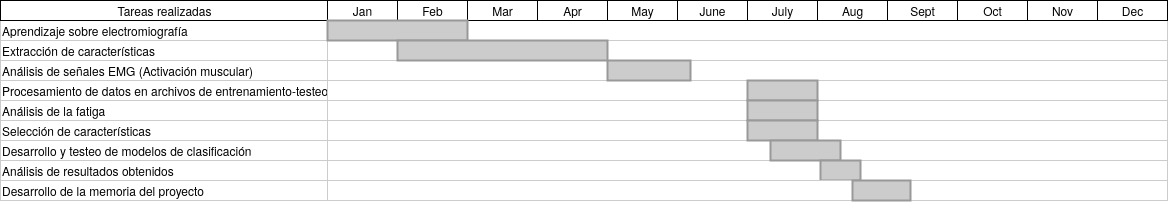
\includegraphics[width=1.0\textwidth,height=4cm]{imagenes/tareas realizadas.png}
\caption{ Diagrama de Gantt sobre el trabajo personal }
\label{fig:gantt}
\end{figure}



\section{Coste}
Una vez realizado el estudio sobre la clasificación y viendo cual sería el mejor clasificador que resolviese el problema, el siguiente paso sería llevarlo al mercado. Habría que realizar una aplicación móvil, conectada a dicho sensor para que mientras se tome los datos, un programa paralelo los analice y nos de los resultados de la fatiga en el tiempo de ejecución, intentando una eficiencia máxima y el mínimo tiempo de procesamiento de datos. Para realizar dicho trabajo los costes se podrían dividir entre el coste de la tecnología utilizada para la obtención de los datos y el coste de los recursos humanos encargados de desarrollar el software.

\subsection{Tecnología utilizada}
Con respecto al precio de la tecnología utilizada, para la medición de los datos se ha utilizado el sensor de mDurance. Se han evaluado ambas rodillas a la hora de realizar una sentadilla por lo que se ha hecho uso del mDurance Premium de 4 canales (Ver Imagen \ref{fig:mDurance}), que además también incluye un sensor para medir el rango de movimiento de cada repetición. Esta herramienta tiene un coste actual de 5.445 \euro \thinspace\thinspace(Enlace a tienda \cite{informacionPreciomdurance}).

\begin{figure}[ht]
\centering
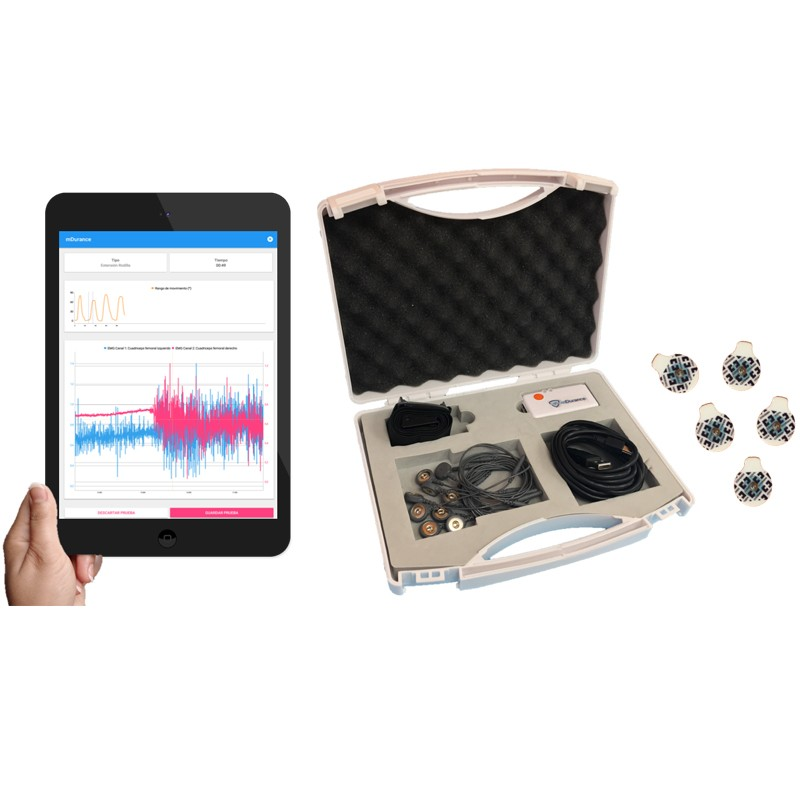
\includegraphics[scale=0.3]{imagenes/electromiografo-de-superficie-de-dos-canales-mdurance-pro.jpg}
\caption{ Electromiógrafo mDurance \cite{electrodosMdurance}}
\label{fig:mDurance}
\end{figure}

\subsection{Recursos humanos}
Para el desarrollo software de la aplicación un ingeniero informático especializado en el desarrollo y la implementación de software cobra unos 2000 \euro/mes  \cite{salarioinformatico}. Estimo que el desarrollo de dicha aplicación se podría llevar a cabo en 2 meses de trabajo, teniendo en cuenta un testeo de funcionamiento para que no requiera un gran mantenimiento al tener la mayoría de errores depurados.

A este precio habría que añadirle lo que cobra un fisioterapeuta/entrenador que será el encargado de tomar los datos a sus clientes. El sueldo medio en España de un fisioterapeuta es de 1217 \euro/mes \cite{salariofisio}.

El precio total de los recursos humanos seria de unos 5217 \euro, debido a dos meses de trabajo del ingeniero informático y a un mes de trabajo del fisioterapeuta encargado de la toma de datos para haber podido realizar el estudio sobre que clasificador es el que obtiene mejores prestaciones.

\subsection{Precio del servicio final}

Todo esto haría un presupuesto final de unos 10662 \euro, un precio bastante elevado, pero si lo analizamos muy rentable, ya que se trata de una herramienta pionera en el sector, que si se desarrolla de la forma adecuada de seguro que sería utilizada por una gran cantidad de atletas y dejaría grandes beneficios.

Este software podría ser implementado dentro de la herramienta base de mDurance, aportando así una funcionalidad extra.


\begin{figure}[ht]
\centering
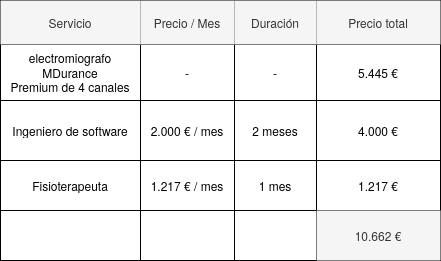
\includegraphics[scale=0.6]{imagenes/precio total.png}
\caption{ Desglose de los precios del proyecto}
\label{fig:precios}
\end{figure}






 %como se ha ido pprogrmamando y llevando a cabo el proyecto
%
\chapter{Análisis del problema \label{analisis}}
Este capítulo está dedicado a una explicación a fondo sobre el análisis del problema. Para ello se comentan los factores más relevantes sobre la fatiga muscular y su detección. Además se comenta un posible caso de lesión en rodillas a la hora de analizar la fatiga.


\section{Fatiga y sistema nervioso central}

La aparición de la fatiga durante la actividad física implica grandes cambios en la realización y percepción del esfuerzo. Esto hace que al realizar varias repeticiones, de por ejemplo en este caso, sentadillas, la acumulación de fatiga haga que cada vez realicemos una peor técnica y debido a esto aumenten las posibilidades de sufrir una lesión \cite{moreno2017fatiga}. Es decir, después de una sesión de entrenamiento, debido a la fatiga, no podemos realizar el mismo esfuerzo muscular y esto aumenta las deficiencias en la musculatura y puede llegar a provocar lesiones si no se trabaja con cuidado.


Otro factor a tener en cuenta, es que ciertos grupos musculares antagonistas pueden entrar en fatiga antes que otros debido a una mayor activación. Esto será tratado más a fondo en la sección de compensación muscular (Ver \ref{compM}). 

La fatiga está muy relacionada con el sistema nervioso central, ya que el sistema nervioso central (Ver \ref{fig:snc}) es el encargado de generar los impulsos eléctricos para que se produzcan las contracciones musculares. Cuanto mayor sean estos impulsos mayor grupo de motoneuronas serán implicadas y un mayor grupo de fibras musculares reclutadas, por lo que se tendrá una mayor fuerza física, así como un mayor control del peso cargado y una mayor técnica. Por ende si el sistema nervioso central está fatigado se tendrá un menor control del peso cargado, menor fuerza y peor técnica. Eso sería la llamada fatiga central, es decir, la fatiga del sistema nerviosos central.

Como bien se comenta en \cite{moreno2017fatiga} esta fatiga todavía es difícil de detectar, pero puede provocar una alteración en la transmisión del sistema nervioso central y en el reclutamiento de los axones motores. Debido a esto, el sujeto que está experimentando dicha fatiga no puede realizar toda la fuerza que sería capaz de realizar en condiciones normales, ya que como se ha explicado antes, no se reciben tantos impulsos para reclutar las fibras musculares. Esto hace que se vea reflejada una caída en la velocidad de ejecución de las sentadillas. Esto es debido a que la velocidad de ejecución y la fuerza realizada están muy relacionadas debido a que cuanto mayor es el número de fibras reclutadas mayor es la fuerza realizada y por consiguiente una mayor velocidad a la hora de realizar las sentadillas. Debido a esto, se ve bastante claro que fatiga y velocidad de ejecución en los entrenamientos son dos términos que están estrechamente relacionados.


\begin{figure}[ht]
\centering
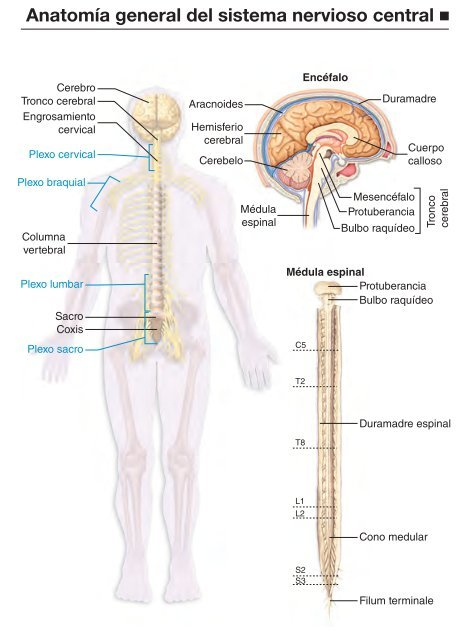
\includegraphics[scale=0.8]{imagenes/SNCcompleto.jpg}
\caption{Sistema nervioso central \cite{imagenSNC}}
\label{fig:snc}
\end{figure}


\newpage
\section{Velocidad de ejecución \label{velo condicion}}
Como bien se ha explicado anteriormente, la fatiga y la velocidad de ejecución son dos términos muy relacionados. Debido a ello un gran número de atletas actuales han basado sus entrenamientos en la velocidad de ejecución. Cuando detectan una caída de velocidad realizan un descanso de la actividad física, para no llegar a niveles muy extremos de fatiga y así poder sacar el máximo partido a sus sesiones de entrenamiento.

Para la detección de esta fatiga se ha estimado que la caída de velocidad de ejecución debe de ser de un 20 por ciento \cite{fernandezpropuesta}. Para ello se tendrá en cuenta dicho porcentaje con respecto a la primera repetición realizada.

A continuación se muestra una tabla-resumen, extraída de los datos utilizados para este proyecto, donde se pueden ver los valores de velocidad de ejecución de las 12 repeticiones registradas junto con el umbral de fatiga resultante. Finalmente una determinación de la fatiga muscular y una conclusión donde el entrenamiento debería de haber sido parado. Para la realización de este proyecto además de la caída del 20 por ciento en la velocidad, se ha estimado que dicha condición se debe de cumplir dos veces seguidas, es decir, en dos repeticiones realizadas consecutivamente, para así eliminar errores y obtener datos más precisos, ya que hay veces que existe caída de velocidad, pero no por fatiga, sino por factores externos, como la falta de concentración del atleta. 


\begin{figure}[ht]
\centering
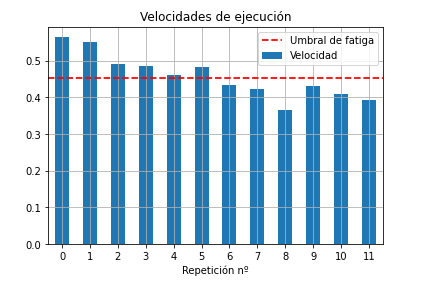
\includegraphics[scale=0.8]{imagenes/velocidades y fatiga.png}
\caption{Velocidad y umbral de fatiga}
\label{fig:fatiga}
\end{figure}

\section{Lesiones y compensación muscular}\label{compM}
Anteriormente se ha comentado que el hecho de realizar esfuerzo físico bajo una gran fatiga puede hacer que nuestros déficits, musculares o articulares aumenten, debido a la perdida de control del sistema nervioso central, y se produzca una lesión.

A parte de esto, en sujetos que ya tienen una lesión en la rodilla, esto se ve más incrementado. Por ejemplo en la lesiones de ligamento cruzado anterior (Ver \ref{fig:lca}), se ha detectado que las personas que la sufren experimentan una serie de cambios en la musculatura de su pierna. En este estudio realizado sobre personas con dicha lesión \cite{kim2018influencia} se demuestra que existe cierta compensación muscular entre los cuádriceps y los isquiotibiales cuando se sufre dicha lesión. Se demuestra que al haber sufrido una rotura del ligamento cruzado anterior, se produce un perdida de fuerza en la musculatura implicada en la rodilla, isquitibiales y cuadriceps. Sin embargo, esta perdida de fuerza es mucho mayor en los cuadriceps que en los isquiotibiales. Esto es  debido a que los pacientes con el ligamento cruzado anterior lesionado, producen una compensación muscular. Se debe a que los cuadriceps son los encargados de la extensión de la rodilla y los isquiotibilaes de la contracción de esta. Por ello, cuando existe dicha lesión, el isquiotibial no deja que el cuadriceps funcione a plenitud, para así, evitar una fuerte extensión de rodilla y evitar producir una gran tensión en el ligamento anterior cruzado, el cual, está dañado.

\begin{figure}[ht]
\centering
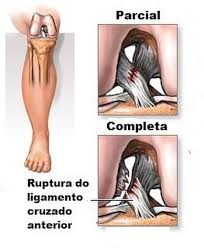
\includegraphics[scale=0.75]{imagenes/lca.jpeg}
\caption{Ligamento cruzado anterior: lesión parcial y completa \cite{imagenLCA}}
\label{fig:lca}
\end{figure}


Para ello la detección de la fatiga mediante diferentes clasificadores que reciban la información de los diferentes músculos examinados, puede ser clave para ver que músculos entran antes en fatiga, y si se produce en el orden correcto. Si no es así, sería un gran indicativo de que existe cierta anomalía en la rodilla. 

Por ejemplo, en la ejecución de una sentadilla, la activación de los cruadriceps debería de ser siempre mucho mayor que la de los isquiotibiales.





 %analisis del problema, fatiga y compensacion en rodillas lesionadas
%
\chapter{Metodología} \label{cap6}
Este capitulo está dedicado a la explicación sobre la metodología del proyecto. Se explica el diseño llevado a cabo a la hora de la extracción y clasificación de las características de la señal EMG. Además se explica el diseño de los 3 tipos de clasificadores que finalmente se han implementado, junto con sus diferentes archivos de entrenamiento-testeo. 

\section{Pipeline del proyecto}
A continuación se muestra un breve resumen junto a un diagrama para mostrar el pipeline del proyecto y facilitar la compresión de la  parte restante del diseño:

\begin{itemize}
\item Obtención de las señales EMG.
\item Una vez obtenidas las señales EMG, pasamos a una fase de extracción de características, donde se extrae información relevante de las señales. 
\item Después de esto se procede con la creación de los diferentes archivos de entrenamiento-testeo que van a ser utilizados y con la estimación de la correspondiente fatiga de cada repetición registrada.
\item El siguiente paso consta de una fase de selección de características de los archivos implementados para obtener así modelos sencillos y eficientes.
\item Finalmente una fase de clasificación de las señales.
\end{itemize}


\begin{figure}[ht]
    \centering
    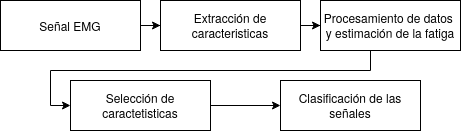
\includegraphics[scale=0.7]{imagenes/diagrma simple.png}
    \caption{ Pipeline del proyecto }
    \label{fig:esuqmemaarchivo}
    \end{figure}
 
\newpage   
\section{Obtención de las señales EMG}
Los datos utilizados para la realización del proyecto han sido tomados y filtrados con el electromiógrafo de mDurance ya comentado en secciones anteriores. Este electromiógrafo consta de 4 canales, por lo que se han podido analizar el rendimiento de 4 músculos, 2 de ellos de la extremidad inferior derecha y otros 2 de la extremidad inferior izquierda. Con esto lo que se ha obtenido son los datos de las señales de electromiografía asociados a unas pruebas. Para la obtención de los datos se tomó un conjunto de personas, que realizaron 6 series de 12 repeticiones de sentadillas con un peso relativo al 70 por ciento del RM (repetición máxima) de cada persona. Las 6 series fueron repartidas en dos días diferentes, es decir, 3 series por día, siendo estos días no consecutivos. 

También se registraron las velocidades de cada repetición. Con las velocidades de cada repetición y partiendo de la condición explicada en el análisis del problema (ver \ref{velo condicion}), se pueden estimar las repeticiones en donde los sujetos experimentaron fatiga y utilizar todos estos datos para el desarrollo de nuestro modelo de clasificación.


\section{Estimación del tamaño de ventana}
Los datos obtenidos comentados anteriormente y facilitados por mDurance, constan de señales de electromiografía brutas. Para obtener información relevante de estas señales EMG primeramente hace falta estimar el tamaño de ventana de cada una de las repeticiones registradas en las señales. 

Para ello se ha hecho uso de un proceso de detección de la actividad muscular a partir de una señal EMG, para así poder detectar fácilmente los tramos de la señal representativos de cada repetición y poder asociar a cada repetición su correspondiente estado de fatiga, analizando su velocidad registrada. Además con el diseño de dividir una señal EMG en sus diferentes activaciones (ventana de activación), nos aseguramos que los datos obtenidos son reales y más precisos, ya que solo tiene el valor de cada repetición y eliminamos el ruido que ha podido ser producido a la hora de situar o quitar el electromiógrafo.

Además se llevó a cabo una selección de los archivos de EMG más útiles, ya que ciertos archivos, vienen con mucho ruido externo y no se llega a detectar las 12 repeticiones claramente.
\section{Extracción de características}
 Una vez se ha estimado el tamaño de ventana de cada una de las repeticiones, el siguiente paso es la extracción de las características de la señal de cada una de las repeticiones registradas. Para ello con la estimación del tamaño de ventana podemos obtener unas características con unos valores muy fiables. 

 Existen un gran número de características, tanto en el dominio del tiempo, como en el dominio de la frecuencia. En este caso se han estudiado 15 características diferentes. (Para la obtención de conocimientos sobre estas características así como sus funciones se ha hecho uso de \cite{romo2007analisis,phinyomark2012feature}).

Con respecto a las características del dominio del tiempo he investigado sobre:

\begin{itemize}
\item Root mean square (RMS) \cite{phinyomark2012feature}:

    \begin{figure}[ht]
        \centering
        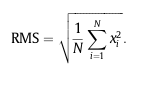
\includegraphics[scale=0.8]{imagenes/formula de caracteristicas/rms.png}
        \caption{ Definición de RMS \cite{phinyomark2012feature}}
        \label{fig:rms1}
    \end{figure}


\item Mean absolute value (MAV) \cite{phinyomark2012feature}:

    \begin{figure}[ht]
        \centering
        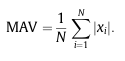
\includegraphics[scale=0.8]{imagenes/formula de caracteristicas/mav.png}
        \caption{ Definición de MAV \cite{phinyomark2012feature}}
        \label{fig:mav1}
    \end{figure}
    
 \newpage   
\item Zero crossing (ZC) con umbral de 0,01 \cite{phinyomark2012feature}:
    \begin{figure}[ht]
        \centering
        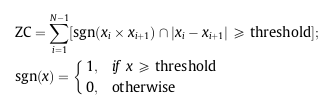
\includegraphics[scale=0.8]{imagenes/formula de caracteristicas/zc.png}
        \caption{ Definición de ZC \cite{phinyomark2012feature}}
        \label{fig:zc1}
    \end{figure}


\item Waveform length (WL) \cite{phinyomark2012feature}:
    \begin{figure}[ht]
        \centering
        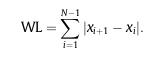
\includegraphics[scale=0.8]{imagenes/formula de caracteristicas/wl.png}
        \caption{ Definición de WL \cite{phinyomark2012feature}}
        \label{fig:wl1}
    \end{figure}

\item Slope sign change (SSC) con umbral de 0,01 \cite{phinyomark2012feature}:
    \begin{figure}[ht]
        \centering
        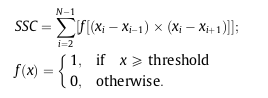
\includegraphics[scale=0.8]{imagenes/formula de caracteristicas/ssc.png}
        \caption{ Definición de SSC \cite{phinyomark2012feature}}
        \label{fig:ssc1}
    \end{figure}
   
\item Integrated EMG (IEMG) \cite{phinyomark2012feature}:
    \begin{figure}[!ht]
        \centering
        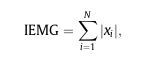
\includegraphics[scale=0.8]{imagenes/formula de caracteristicas/iemg.png}
        \caption{ Definición de IEMG \cite{phinyomark2012feature}}
        \label{fig:iemg1}
    \end{figure}
\newpage
\item Simple square integral (SSI) \cite{phinyomark2012feature}:
    \begin{figure}[!ht]
        \centering
        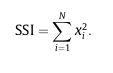
\includegraphics[scale=0.8]{imagenes/formula de caracteristicas/ssi.png}
        \caption{ Definición de SSI \cite{phinyomark2012feature}}
        \label{fig:ssi1}
    \end{figure}
    

\item Variance of EMG (VAR) \cite{phinyomark2012feature}:
    \begin{figure}[ht]
        \centering
        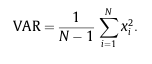
\includegraphics[scale=0.8]{imagenes/formula de caracteristicas/var.png}
        \caption{ Definición de VAR \cite{phinyomark2012feature}}
        \label{fig:var1}
    \end{figure}
    
    
    
\item Absolute value 3rd (TM3) \cite{phinyomark2012feature}:
    \begin{figure}[!ht]
        \centering
        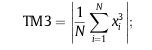
\includegraphics[scale=0.8]{imagenes/formula de caracteristicas/tm3.png}
        \caption{ Definición de TM3 \cite{phinyomark2012feature}}
        \label{fig:tm31}
    \end{figure}
    

\item Absolute value 4th (TM4) \cite{phinyomark2012feature}:
    \begin{figure}[!ht]
        \centering
        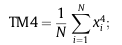
\includegraphics[scale=0.8]{imagenes/formula de caracteristicas/tm4.png}
        \caption{ Definición de TM4 \cite{phinyomark2012feature}}
        \label{fig:tm41}
    \end{figure}
\item Absolute value 5th (TM5) \cite{phinyomark2012feature}:
    \begin{figure}[!ht]
        \centering
        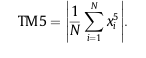
\includegraphics[scale=0.8]{imagenes/formula de caracteristicas/tm5.png}
        \caption{ Definición de TM5 \cite{phinyomark2012feature}}
        \label{fig:tm51}
    \end{figure}
    
\newpage
\item Log detector (LOG) \cite{phinyomark2012feature}:
    \begin{figure}[!ht]
        \centering
        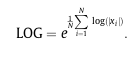
\includegraphics[scale=0.8]{imagenes/formula de caracteristicas/log.png}
        \caption{ Definición de LOG \cite{phinyomark2012feature}}
        \label{fig:log1}
    \end{figure}
    
\item Average amplitude change (ACC) \cite{phinyomark2012feature}:
    \begin{figure}[!ht]
        \centering
        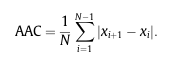
\includegraphics[scale=0.8]{imagenes/formula de caracteristicas/acc.png}
        \caption{ Definición de ACC \cite{phinyomark2012feature}}
        \label{fig:acc1}
    \end{figure}
\end{itemize}

Con respecto al dominio de la frecuencia he investigado sobre:
\begin{itemize}
\item Median frecuency (MDF) \cite{phinyomark2012feature}:
    
    \begin{figure}[!ht]
        \centering
        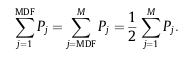
\includegraphics[scale=0.8]{imagenes/formula de caracteristicas/mdf.png}
        \caption{ Definición de MDF \cite{phinyomark2012feature}}
        \label{fig:mdf1}
    \end{figure}

\item Mean frecuency (MNF) \cite{phinyomark2012feature}:
    \begin{figure}[!ht]
        \centering
        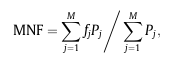
\includegraphics[scale=0.8]{imagenes/formula de caracteristicas/mnf.png}
        \caption{ Definición de MNF \cite{phinyomark2012feature}}
        \label{fig:mnf1}
    \end{figure}
\end{itemize}

\newpage
\section{Estimación de fatiga}
Para estimar la fatiga, como ya se ha comentado en capítulos anteriores, el proyecto se ha basado en que una vez que se registra una velocidad que decae un 20 por ciento, con respecto a la velocidad de la primera repetición y esto se cumple en dos repeticiones seguidas, se considera que el atleta ha entrado en fatiga y la repetición en cuestión analizada y todas las siguientes se etiquetarán como fatiga.


\section{Selección de características: RFE}
Para dotar al clasificador de una mayor simpleza y un mejor rendimiento tanto a la hora de clasificar como en tiempo de ejecución, se ha utilizado un algoritmo para estimar que características de todas las estudiadas anteriormente son las más representativas de la fatiga. Se ha hecho uso del algoritmo Recursive Feature Elimination (RFE) \cite{ramos2018emg}. Este algoritmo parte del dataset completo y en cada iteración elimina la característica menos representativa, hasta que se alcanza el número de características deseado. Con el uso de este algoritmo se han obtenido tres tipos de dataset con diferente número de variables para realizar el estudio. En este caso fueron estudiados con 1 característica, con 2 características y con 5 características. Por lo que finalmente obtendremos un gran número de resultados para realizar las conclusiones oportunas. El esquema final de todos los dataset que serán analizados es el siguiente (Ver \ref{fig:esquemageneral}).


\section{Clasificación binaria de señales}
Una vez realizada toda la fase de extracción y selección de características, debemos de realizar el diseño de los clasificadores. Para nuestro problema de clasificación binaria, donde 1 es identificador de fatiga y 0 es identificador de no fatiga, hemos estudiado el rendimiento de tres clasificadores. Se trata de 3 conjuntos de algoritmos de aprendizaje supervisado donde es necesario un conjunto de datos para el entrenamiento del modelo y otro conjunto de datos no conocido por el modelo, para estudiar su rendimiento a la hora de clasificar. A continuación se explica el funcionamiento y diseño de cada uno de ellos.
    \newpage
    \subsection{Support vector machines (SVMs): máquinas de vector de soporte}
    Su clasificación reside en que se construye un modelo que es capaz de predecir a que subgrupo de los dos, pertenece un nuevo punto del cual no conocemos su categoría.
    Para ello lo que se realiza es la obtención de un hiperplano que divida el conjunto de datos iniciales en dos grupos bien diferenciados. Los vectores de soporte son los encargados de definir el espacio de separación entre el hiperplano y las dos clases en cuestión (1,0). Cuanto mayor sea el margen entre los vectores de soporte de cada clase y el hiperplano, mejor será el modelo, ya que tendrá más claro donde clasificar datos futuros. Para el diseño del modelo se ha utilizado el kernel tipo sigmoide.
    
    \begin{figure}[ht]
    \centering
    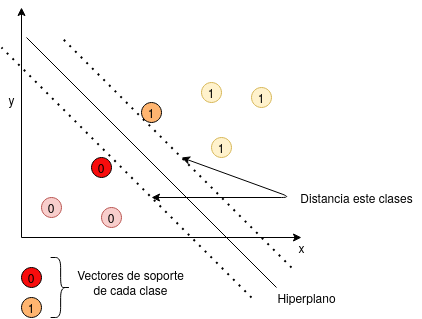
\includegraphics[width=1.0\textwidth]{imagenes/svm.png}
    \caption{ Esquema sobre funcionamiento del clasificador SVM }
    \label{fig:svm}
    \end{figure}
    
    \newpage
    \subsection{Decision trees (Trees): árboles de decisión}
    Los árboles de decisión son unos de los métodos más populares en machine learning debido a su gran eficiencia y sencillez. Se trata de un algoritmo de aprendizaje supervisado. Se puede entender como un árbol general formado por subárboles, donde cada nodo raíz de cada subárbol es una condición y las hojas de dichos subárboles, las etiquetas. El algoritmo selecciona las características del dataset más influyentes y va dividiendo el dataset completo en subconjuntos de datos, por lo que, dichas características formarán parte de los nodos de decisión, hasta que todos los nodos del árbol sean nodos hoja.
    
    
    \begin{figure}[!ht]
    \centering
    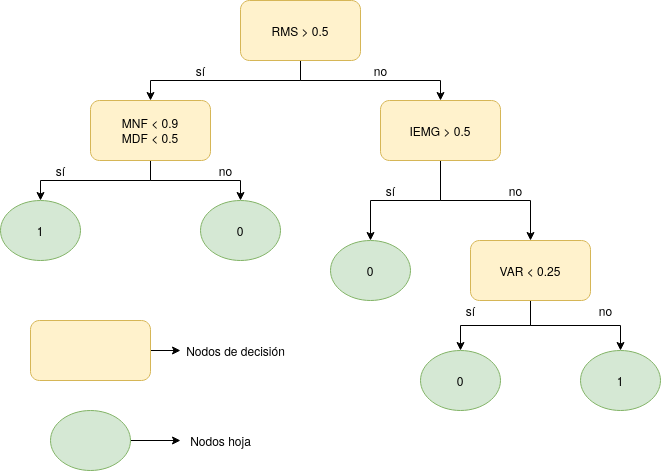
\includegraphics[width=1.0\textwidth]{imagenes/arboles de decision.png}
    \caption{ Esquema sobre funcionamiento del árbol de decisión }
    \label{fig:arbol}
    \end{figure}
    
 
  
    \subsection{K nearest neighbors (KNN): K vecinos más cercanos}
    Este algoritmo de clasificación opera de una forma muy sencilla. Se basa en estimar la categoría de un dato nuevo, en base a la categoría de sus K vecinos más cercanos. De estos K vecinos más cercanos sí conoce su categoría debido a que forman parte del conjunto de datos de entrenamiento. Debido a esto el valor de K que sea utilizado influirá mucho en el rendimiento de nuestro clasificador. El valor de K que se ha utilizado para este proyecto es de 6 vecinos.
    \begin{figure}[!ht]
    \centering
    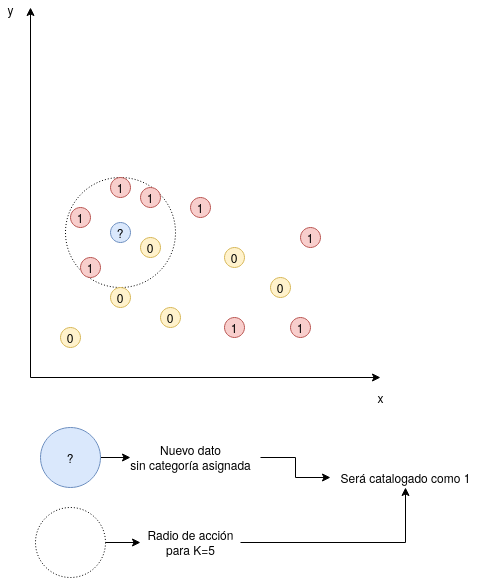
\includegraphics[width=1.0\textwidth]{imagenes/KNN.png}
    \caption{ Esquema sobre funcionamiento del KNN para K = 5 }
    \label{fig:knn}
    \end{figure}
    \section{Estudio del rendimiento obtenido: validación cruzada}
    Para validar el rendimiento de los tres clasificadores expuestos anteriormente se ha hecho uso de la validación cruzada. Con esto, sobre un mismo archivo de entrenamiento-testeo obtenemos diferentes conjuntos de datos para evaluar y testear el clasificador. En cada iteración el modelo se entrena con una parte diferente del conjunto de datos del archivo entrenamiento-testeo y con la parte restante se realiza el testeo. (Ver \ref{fig:validacioncruzada}).
    
    Se obtendrá una serie de precisiones, una por cada iteración de la validación cruzada, y podremos obtener una precisión media del clasificador y una desviación estándar, que nos dará una idea de cuanto de bueno es nuestro clasificador. Para el diseño de nuestra validación cruzada se ha utilizado un valor de k = 15.
    
    \begin{figure}[ht]
    %\centering
    \includegraphics[width=1.0\textwidth, height=10cm]{imagenes/validación cruzada.png}
    \caption{ Validación cruzada para k = 5  }
    \label{fig:validacioncruzada}
    \end{figure}
    
    
\section{Procesamiento de datos: diferentes modelos de estudio} \label{tiposClasificadores}
El electromiógrafo utilizado para la medición de la actividad muscular a la hora de realizar las sentadillas consta de 4 canales diferentes. (Ver Imagen \ref{fig:esquemaarchivoEMG}).
\begin{itemize}
\item Canal 1: registra la actividad muscular del vasto medial de la pierna izquierda.
\item Canal 2: registra la actividad muscular del recto femoral de la pierna izquierda.
\item Canal 3: registra la actividad muscular del vasto medial de la pierna derecha.
\item Canal 4: registra la actividad muscular del recto femoral de la pierna derecha.
\end{itemize}
Debido a la gran ventaja que nos aporta la herramienta utilizada se ha optado por realizar diferentes tipos de archivos de entrenamiento-testeo y ver cual de ellos sería el más indicado a la hora de resolver nuestro problema. Cada uno de los archivos de entrenamiento-testeo que se van a describir a continuación están formados mediante la agrupación de los diferentes canales. Con esto se pretende simular diferentes situaciones y ver cual de ellas sería la más indicada para resolver el proyecto.



A continuación se muestra un esquema resumen sobre los archivos EMG utilizados y sus características extraídas. Con estos datos se formarán los archivos de entrenamiento-testeo.


    \begin{figure}[!ht]
    \centering
    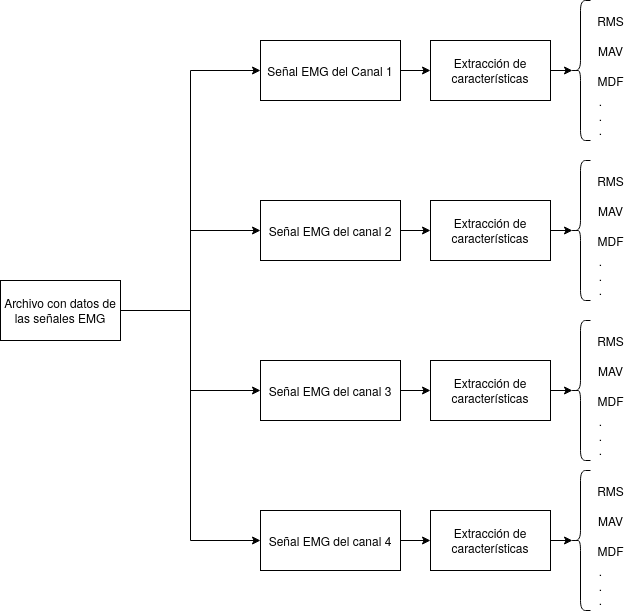
\includegraphics[width=0.94\textwidth]{imagenes/esquema de los canales.png}
    \caption{ Esquema de archivo EMG bruto: 1 serie de 12 repeticiones de sentadillas }
    \label{fig:esquemaarchivoEMG}
    \end{figure}



    \subsection{Canal 1, canal 2, canal 3, canal 4}
La primera idea llevada a cabo es implementar un clasificador para cada canal. Con esto lo que se obtendría es una precisión muscular muy alta a la hora de detectar la fatiga muscular. Es decir, a la hora de realizar una serie de sentadillas podríamos averiguar que músculo de los 4 registrados es el que entra en fatiga. Para ello se han diseñado 4 tipos de archivos de entrenamiento-testeo. Los 4 tipos de archivos tienen la misma organización, lo único que cambia entre ellos es el valor que contienen. Por ejemplo, el archivo del canal 1, solo contiene los valores de las características extraídas de las señales EMG del vasto medial izquierdo. Para ello cada columna del dataset es identificada por cada una de las 15 características estudiadas, siendo la última columna, la representación de la fatiga asociada a cada repetición. Con respecto a las filas, las 12 primeras filas corresponden a las 12 repeticiones del primer archivo EMG analizado, las 12 siguientes a las 12 repeticiones del segundo archivo, etc. 

Esto se puede aplicar también a los canales 2, 3 y 4. El esquema para el archivo de entrenamiento-testeo del canal N siendo N={1, 2, 3, 4} y de cada archivo K siendo K={1, 2, ..., 19} (número total de archivos analizados) es:

\begin{figure}[ht]

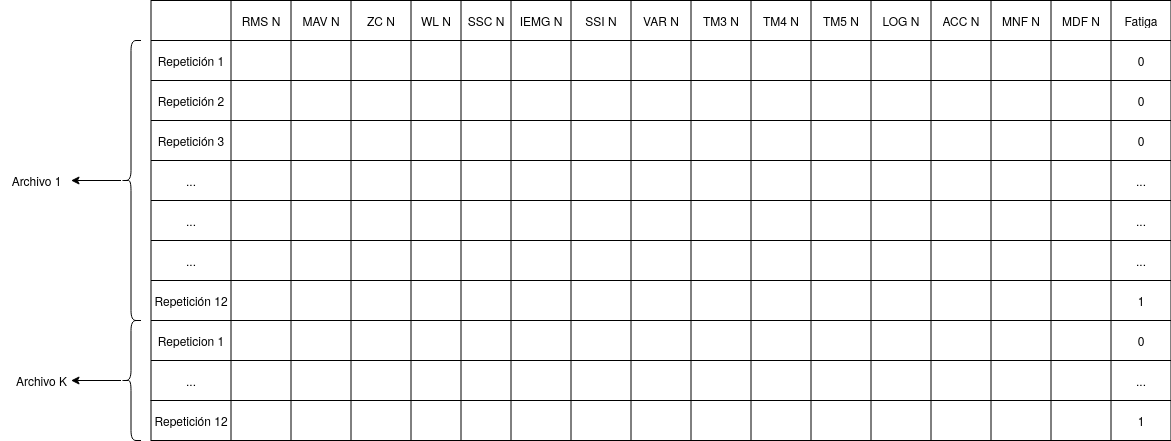
\includegraphics[width=1.0\textwidth,height=7cm]{imagenes/canal1234.png}
\caption{ Esquema de archivo de entrenamiento-testeo para cada canal 1, 2, 3, 4}
\label{fig:canal1234}
\end{figure}


\newpage
    \subsection{Canal 1,2 y canal 3,4}
Debido a que la sentadilla es un ejercicio multiarticular e implica a las dos extremidades inferiores, la segunda idea consta de diseñar un clasificador para cada extremidad. Con esto tendremos un nivel de especificidad a nivel de extremidad y podremos detectar que extremidad inferior se fatiga antes, si la izquierda o la derecha. Para ello en esta ocasión tenemos dos archivos de entrenamiento-testeo, uno de cada extremidad. Lo que se ha llevado a cabo es la agrupación de los datos recolectados por el canal 1 y canal 2 (extremidad izquierda) y por el canal 3 y canal 4 (extremidad derecha). A continuación se muestra una breve explicación de cada archivo, así como su correspondiente esquema.

        \subsubsection{Canal 1,2: extremidad izquierda}
        Como se ha comentado anteriormente, este archivo de entrenamiento-testeo consta de los datos agrupados del canal 1 y del canal 2. En este caso el número de filas aumenta, ya que tratamos las repeticiones del canal 1 y las repeticiones del canal 2. Su esquema es el siguiente (Ver \ref{fig:canal12}).
        
        \begin{figure}[!ht]
        
        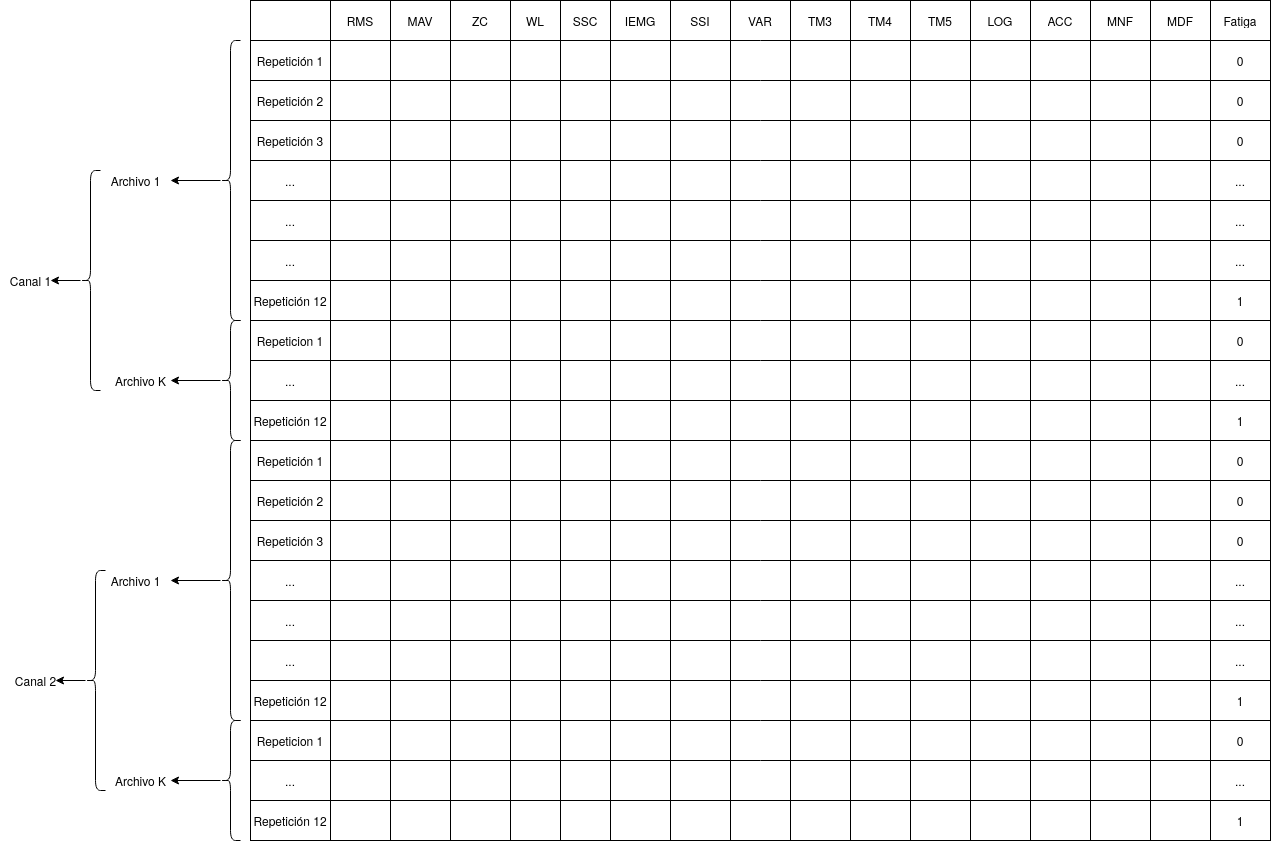
\includegraphics[width=1.0\textwidth,height=9cm]{imagenes/canal 12.png}
        \caption{ Esquema de archivo de entrenamiento-testeo para el canal 1,2}
        \label{fig:canal12}
        \end{figure}
        
        
        \newpage
        \subsubsection{Canal 3,4: extremidad derecha}
        El archivo de entrenamiento-testeo del clasificador de la extremidad derecha, es similar al de la extremidad izquierda. La única diferencia es que en este caso se agrupan los datos del canal 3 y del canal 4. Su esquema es el siguiente (Ver \ref{fig:canal34}).
        \begin{figure}[!ht]
        \centering
        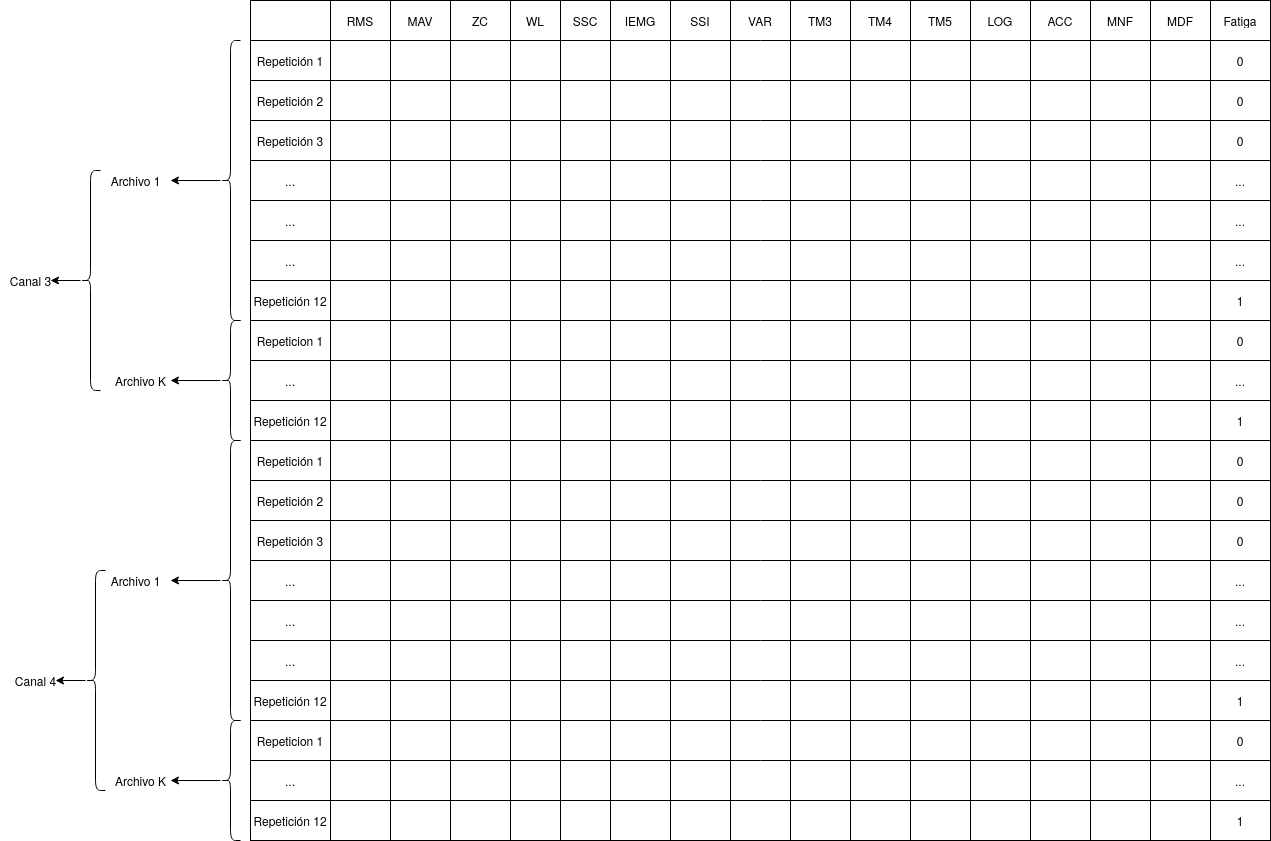
\includegraphics[width=1.0\textwidth,height=9cm]{imagenes/canal 34.png}
        \caption{ Esquema de archivo de entrenamiento-testeo para el canal 3,4}
        \label{fig:canal34}
        \end{figure}
        
    
    
    \subsection{Canal total}
    Por último, se ha pensado en el diseño de un clasificador que ha sido denominado total, donde se hallará la fatiga global del individuo en cuestión. Para ello se agruparán los datos de los 4 canales utilizados en un mismo archivo de entrenamiento-testeo. En este caso el número de filas aumenta, debido a que tenemos en conjunto la información de todos los canales. El esquema de dicho archivo es el siguiente (Ver \ref{fig:canaltotal}).


    \begin{figure}[ht]
    \centering
    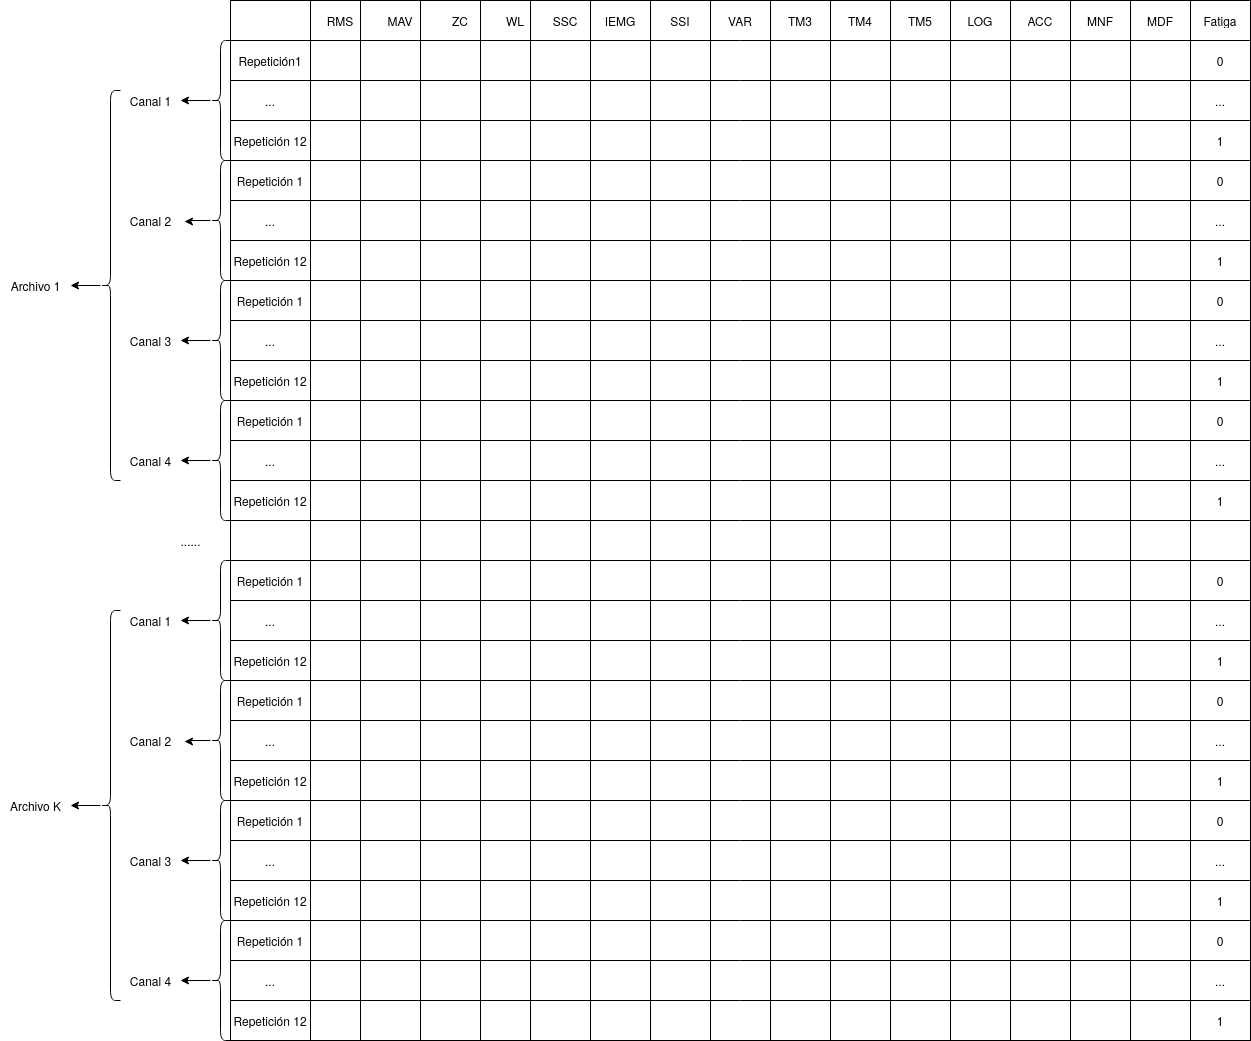
\includegraphics[scale=0.28]{imagenes/canal total.png}
    \caption{ Esquema de archivo de entrenamiento-testeo para el canal total }
    \label{fig:canaltotal}
    \end{figure}

    
        \newpage
    
\section{Esquema final del estudio}
Para finalizar la fase de metodología se pretende mostrar un esquema final sobre los diferentes tipos de clasificadores finales. El objetivo es analizar cuál sería el número óptimo de características (N=1,2,5 ) y el tipo de clasificador (SVM, Tree, KNN) para cada uno de los canales que son estudiados (canal 1, canal 2, canal 3, canal 4, canal (1,2), canal (3,4), canal total). Ver sección \ref{tiposClasificadores} para mayor detalle. (Ver esquema \ref{fig:esquemageneral}).



 \begin{figure}[h]
    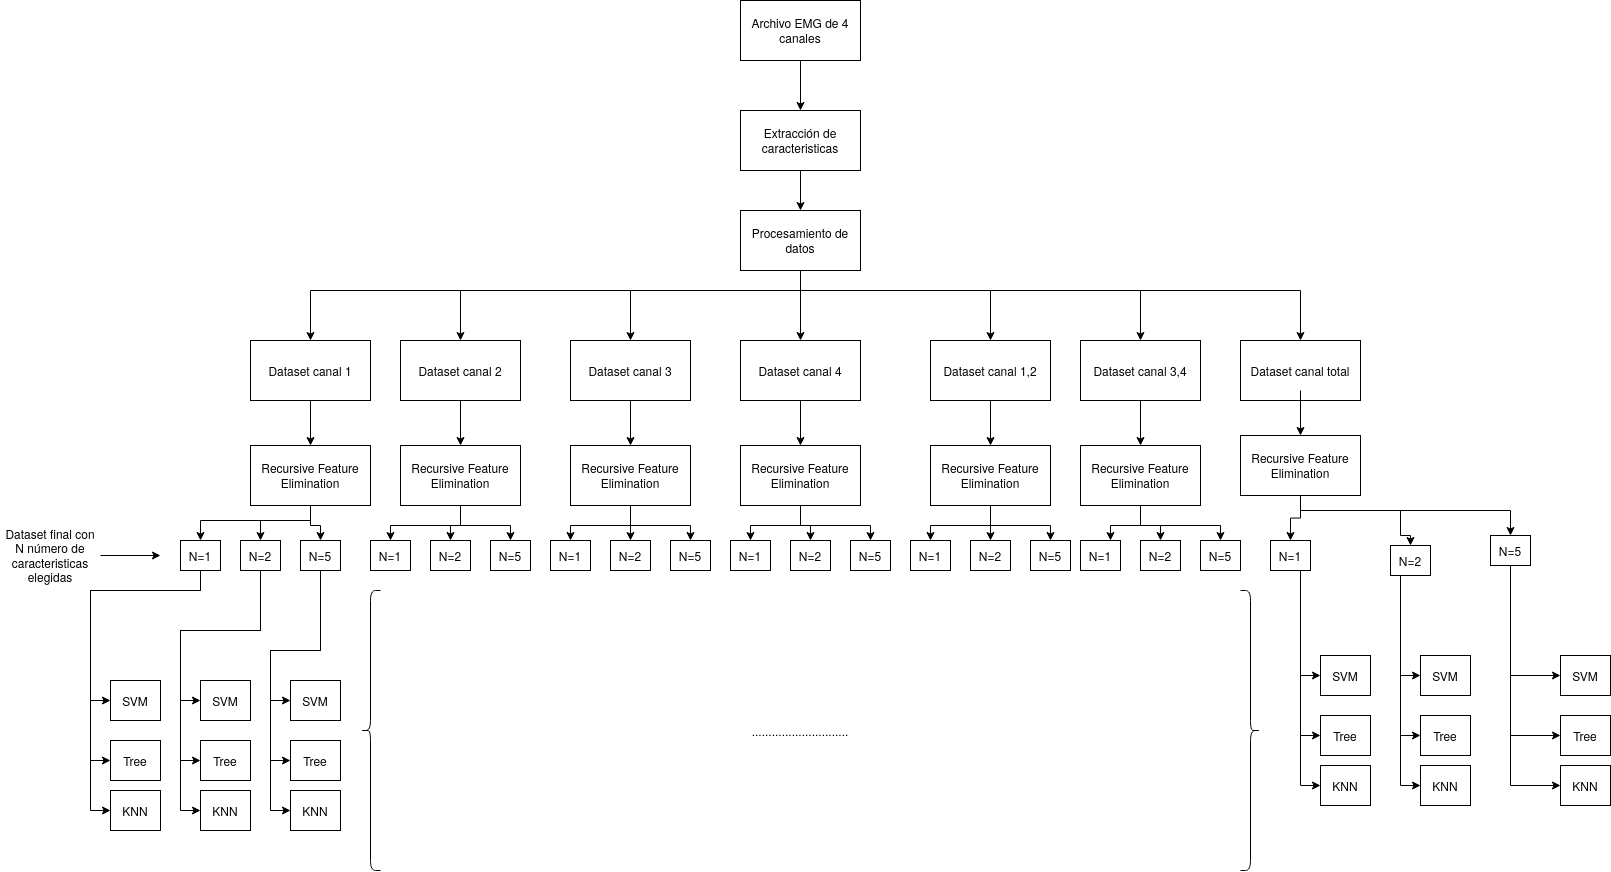
\includegraphics[height=0.85\textwidth,angle=90]{imagenes/esquema final.png}
    \caption{ Esquema general del sistema }
    \label{fig:esquemageneral}
   \end{figure}
    

 %diseño de los dataset y de los tres tipos de clasificadores, extraccion y seleccion de caracteristicas, clasificadores ,,,,normalmente a través de diagramas y texto que ayude a explicar la secuencia de operación del sistema
%
\chapter{Implementación}
Este capítulo está dedicado a la implementación realizada del proyecto. Tiene una estructura muy similar a la del capítulo \ref{cap6}, solo que en dicho capítulo se habla sobre el diseño y la metodología del proyecto y este está dedicado a su implementación en Python 3 \cite{python}.
Para su desarrollo se han utilizado los notebooks de Jupyter \cite{jupyter}. Jupyter es una aplicación web de código abierto, que permite crear documentos donde se incluyen ecuaciones, texto, código, gráficas, etc. Además es compatible con una gran cantidad de bibliotecas de machine learning y procesamiento de datos.

Las bibliotecas de ciencia de datos utilizadas para el desarrollo de este proyecto han sido:
\begin{itemize}
\item pandas: utilizada para el tratamiento y el análisis de los datos tratados. De gran utilidad con sus dataFrames para organizar los datos y exportarlos e importarlos en sus correspondientes .csv \cite{pandas}.
\end{itemize}
\begin{lstlisting}
import pandas as pd
\end{lstlisting}

\begin{itemize}
\item numpy: librería que añade funcionalidad a Python con un gran aporte sobre matrices y vectores. Es complementaria a pandas y de gran utilidad en conjunto \cite{numpy}.
\end{itemize}
\begin{lstlisting}
import numpy as np
\end{lstlisting}


Para el procesamiento de señales se ha utilizado:
\begin{itemize}
\item scipy: librería especializada en matemáticas, ciencia e ingeniería. Aporta diversos módulos especializados en diversos temas. El más utilizado en este proyecto fue signal, utilizada para el procesamiento de señales (FFT, PSD, welch) \cite{scipy,scipysignal}.
\end{itemize}

\begin{lstlisting}
import scipy as sp
from scipy import signal
from scipy.fftpack import rfft,rfftfreq
\end{lstlisting}

Para dibujar las diferentes gráficas obtenidas se ha hecho uso de:
\begin{itemize}
\item matplotlib: aporta la funcionalidad para la visualización de los datos procesados con Python \cite{matplotlib}.
\end{itemize}

\begin{lstlisting}
import matplotlib.pyplot as plt
\end{lstlisting}

Para el procesamiento de archivos:
\begin{itemize}
\item glob: aporta la funcionalidad para abrir la base de datos utilizada y examinar cada uno de los archivos que la forman.
\end{itemize}

\begin{lstlisting}
import glob
\end{lstlisting}

Para la parte de machine learning del proyecto se ha utilizado la biblioteca de pyhton:
\begin{itemize}
\item scikit-learn: aporta una gran funcionalidad con una gran cantidad de algoritmos relacionados con el machine learning \cite{scikit}.
\end{itemize}


El resto de módulos relacionados con scikit-learn, como por ejemplo, para los clasificadores, selección de características y rendimiento, serán explicados en sus correspondientes secciones. Esto fue una breve introducción con las bibliotecas generales.


\section{Estimación del tamaño de ventana}
El proceso dedicado a la estimación del tamaño de ventana se ha realizado con el uso de la biblioteca de biosignalsnotebooks \cite{biosignal}.

\begin{lstlisting}
import biosignalsnotebooks as bsnb
\end{lstlisting}

Para dicho proceso, con el uso de la función:
\begin{lstlisting}
activacion1=bsnb.detect_emg_activations(vastoMedialIzquierdo,fs,smooth_level=smooth,threshold_level=threshold,time_units=False,volts=False, resolution=None,plot_result=plot)
\end{lstlisting}

se obtiene un array con todos los intervalos donde se ha detectado actividad muscular en el archivo de EMG bruto. Con esto ya tenemos el tamaño de ventana de cada repetición y podemos continuar con la extracción de características con dicho tamaño de ventana. Cabe destacar que cada repetición de sentadilla puede tener un tamaño de  ventana diferente.

Por último antes de seguir con la fase de extracción de características, habría que señalar el proceso de selección de los archivos brutos de EMG mejor definidos. Esto es debido a que había ciertos archivos donde claramente no había 12 repeticiones registradas o donde había demasiado ruido y el algoritmo utilizado no detectaba claramente las 12 repeticiones, por lo que opté, por implementar un código donde se examinan todos los archivos definidos con diferentes valores de threshold y de smooth, para así hallar cual sería el par de valores más adecuado a cada archivo de EMG y utilizar dichos archivos junto con su par de valores "threshold, smooth" para la extracción de características. A continuación se muestra la función que realiza dicho procedimiento:



\begin{lstlisting}[language=Python]
def hallarArchivosEMG():
    
    fs=1024
    dataset=glob.glob("../Estudio tDCS/*.csv")
    dataset.sort()

    archivosFinales=[]
    archivos=[]
    valoresSM=[22,21,20,19,18,17,16,15,14]
    valoresTH=[60,57,55,52,50,47,45,42,40,
    37,35,32,30,27,25,22,20,19,18,17,16,15,14,13,12,11,10]
    
    for sm in valoresSM:
        
        for th in valoresTH:

            for archivo in dataset:

                if archivo not in archivos:

                    df = pd.read_csv(archivo,delimiter=";",decimal=",")
                    df=df.fillna(0)

                    #Pierna izquieda
                    vastoMedialIzquierdo= df['emg_muscle_1_(µV)'].to_numpy()
                    rectoFemoralIzquierdo=df['emg_muscle_2_(µV)'].to_numpy()

                    #Pierna derecha
                    vastoMedialDerecho=df['emg_muscle_3_(µV)'].to_numpy()
                    rectoFemoralDerecho=df['emg_muscle_4_(µV)'].to_numpy()


                    #Atributos para detectar EMG
                    plot=False
                    smooth=sm
                    threshold=th

                    activacion1=bsnb.detect_emg_activations(vastoMedialIzquierdo,fs,smooth_level=smooth, threshold_level=threshold, time_units=False,volts=False, resolution=None,plot_result=plot)
                    
                    if (len(activacion1[0]) != 12):
                        continue
                    
                    activacion2=bsnb.detect_emg_activations(rectoFemoralIzquierdo,fs,smooth_level=smooth, threshold_level=threshold,
time_units=False,volts=False, resolution=None,plot_result=plot)

                    if (len(activacion2[0]) != 12):
                        continue
                    
                    activacion3=bsnb.detect_emg_activations(vastoMedialDerecho,fs,smooth_level=smooth, threshold_level=threshold,
time_units=False,volts=False, resolution=None,plot_result=plot)
                    
                    if (len(activacion3[0]) != 12):
                        continue
                    activacion4=bsnb.detect_emg_activations(rectoFemoralDerecho,fs,smooth_level=smooth, threshold_level=threshold,
time_units=False,volts=False, resolution=None,plot_result=plot)
                    if (len(activacion4[0]) != 12):
                        continue

                    datosImportantes=[]
                    datosImportantes.append(archivo)
                    datosImportantes.append(threshold)
                    datosImportantes.append(smooth)
                    archivos.append(archivo)

                    archivosFinales.append(datosImportantes)
    
    return archivosFinales
    
\end{lstlisting}

\section{Extracción de características}
Después de analizar todos los archivos disponibles y realizar su correspondiente estimación de los valores de ventana, podemos proceder a comentar la siguiente fase, la fase de extracción de características. Para la implementación de cada característica me he basado en la función que la define y la he implementado sobre Python. Se aconseja visitar el anexo para ver el código implementado asociado a cada característica. (Ver \ref{anexocaracImple}).


\section{Estimación de fatiga}
Para la estimación de la fatiga comentada, se obtienen las etiquetas de fatiga experimentada, representadas por 1, y fatiga no experimentada, representadas por 0, con el siguiente código. Su funcionamiento es recibir las velocidades de cada una de de las repeticiones registradas y hallar el valor de la etiqueta de la fatiga, basándose en un umbral de caída de velocidad, el cuál viene dado por una caída del 20 por ciento en la velocidad con respecto a la primera repetición.

\begin{lstlisting}
def calculoDeFatiga(velocidad):
    fatiga=[]
    
    umbral=0.8*velocidad[0]
    c=0
    for i in range(0,10):
        c=c+1
        if ((velocidad[i] <= umbral) and (velocidad[i+1] <= umbral) ):
            for j in range(i,12):
                fatiga.append(1)
            
            return np.asarray(fatiga)
        
        else:
            fatiga.append(0)
            
        
    if (len(fatiga) != 12):
        if ((velocidad[c] <= umbral) and (velocidad[c+1] <= umbral)):
            for i in range(len(fatiga),12):
                fatiga.append(1)
        else:
            for i in range(len(fatiga),12):
                fatiga.append(0)
    
    return np.asarray(fatiga)
\end{lstlisting}

\section{Selección de características: RFE}
Como se ha explicado en la fase de diseño, el algoritmo utilizado para la selección de las características más representativas de la fatiga y así obtener unos modelos más sencillos ha sido el Recursive Feature Elimination (RFE). Para su desarrollo se ha hecho uso de la biblioteca scikit-learn de Python con su módulo de selección de características \cite{rfecv}.

A cada uno de los archivos de entrenamiento-testeo de cada canal se le aplica dicho algoritmo, y se extraen 3 archivos de entrenamiento-testeo para cada canal, cada uno con un número diferente de características. 

    \subsection{Canal 1, canal 2, canal 3, canal 4}
Aplicación del RFE a los archivos de entrenamiento-testeo de los canales 1, 2, 3 y 4 con valores de N = 1, 2, 5, donde N es el número de características finales del modelo.
\begin{lstlisting}
caracteristicas=['RMS','MAV','ZC','WL','SSC','IEMG','SSI','VAR','TM3','TM4','TM5','LOG','ACC','MNF','MDF']
#[0] -> N=1 canal 1
#[1] -> N=1 canal 2
#[2] -> N=1 canal 3
#[3] -> N=1 canal 4

#[4] -> N=2 canal 1
#[5] -> N=2 canal 2
#[6] -> N=2 canal 3
#[7] -> N=2 canal 4

listaDeAtributos=[]
numeroCaracteristicas=[1,2,5]


for i in numeroCaracteristicas:
    canal=1
    #Recorro la lista con los valores de los 4 canales
    for dato in datos1234:

        x=dato.to_numpy()
        y=valores1234['fatiga'].to_numpy()

        
        estimator = SVC(kernel="linear")
    
        print("N = " + str(i) + " ------------------------------------------------")
        print("estimacion canal : " + str(canal))

        selector= RFECV(estimator,step=1,cv=15,min_features_to_select=i)
        selector=selector.fit(x,y)

        ni=np.array(selector.support_)
        pi=pd.DataFrame(data=ni,columns=['Validez'])

        pi['Caracteristica']=caracteristicas
        pi['canal']=canal
        pi = pi.drop(pi[pi.Validez == False].index)

        print(pi)
        print("\n\n")

        listaDeAtributos.append(pi['Caracteristica'])
        #listaDeAtributos.append(pi)

        canal=canal+1

#obtengo el dataset para cada clasificador
datosFinales1234=[]

i=0
for caracteristicas in listaDeAtributos:
    if (i > 3):
        i=0
        
    p=pd.DataFrame()
    for caracteristica in caracteristicas:
        p[caracteristica + str(i+1)]=valores1234[caracteristica + str(i+1)]
    i=i+1

    p=(p-p.min())/(p.max()-p.min())
    datosFinales1234.append(p)
\end{lstlisting}



    \subsection{Canal 1,2 y canal 3,4}
        \subsubsection{Canal 1,2}
Aplicación del RFE al archivo de entrenamiento-testeo del canal 1, 2 con valores de N = 1, 2, 5, donde N es el número de características finales del modelo.
\begin{lstlisting}
caracteristicas=['RMS','MAV','ZC','WL','SSC','IEMG','SSI','VAR','TM3','TM4','TM5','LOG','ACC','MNF','MDF']

numeroCaracteristicas=[1,2,5]

RFEcanal12=[]



for i in numeroCaracteristicas:
    
    
    x = valores12.drop(['fatiga'],axis=1).to_numpy()
    y = valores12['fatiga'].to_numpy()

    estimator= SVC(kernel='linear')

    selector= RFECV(estimator,step=1,cv=15,min_features_to_select=i)
    selector=selector.fit(x,y)
    ni=np.array(selector.support_)

    pi=pd.DataFrame(data=ni,columns=['Validez'])

    pi['Caracteristica']=caracteristicas

    pi = pi.drop(pi[pi.Validez == False].index)

    
    print("N= " + str(i))
    print(pi)
    print("\n\n")


    datosFinalesTotales=pd.DataFrame()
    for caracteristica in pi['Caracteristica']:
        datosFinalesTotales[caracteristica]=valores12[caracteristica]


    RFEcanal12.append(datosFinalesTotales)


RFEcanal12
\end{lstlisting}

        \subsubsection{Canal 3,4}
Aplicación del RFE al archivo de entrenamiento-testeo del canal 3, 4 con valores de N = 1, 2, 5, donde N es el número de características finales del modelo.
\begin{lstlisting}
caracteristicas=['RMS','MAV','ZC','WL','SSC','IEMG','SSI','VAR','TM3','TM4','TM5','LOG','ACC','MNF','MDF']

numeroCaracteristicas=[1,2,5]

RFEcanal34=[]

for i in numeroCaracteristicas:
    
    x = valores34.drop(['fatiga'],axis=1).to_numpy()
    y = valores34['fatiga'].to_numpy()

    estimator= SVC(kernel='linear')

    selector= RFECV(estimator,step=1,cv=15,min_features_to_select=i)
    selector=selector.fit(x,y)
    ni=np.array(selector.support_)

    pi=pd.DataFrame(data=ni,columns=['Validez'])

    pi['Caracteristica']=caracteristicas

    pi = pi.drop(pi[pi.Validez == False].index)

    
    print("N= " + str(i))
    print(pi)
    print("\n\n")

    
    datosFinalesTotales=pd.DataFrame()
    for caracteristica in pi['Caracteristica']:
        datosFinalesTotales[caracteristica]=valores34[caracteristica]


    RFEcanal34.append(datosFinalesTotales)


RFEcanal34
\end{lstlisting}
\newpage
    \subsection{Canal total}
Aplicación del RFE al archivo de entrenamiento-testeo del canal total con valores de N = 1, 2, 5, donde N es el número de características finales del modelo.
\begin{lstlisting}
caracteristicas=['RMS','MAV','ZC','WL','SSC','IEMG','SSI','VAR','TM3','TM4','TM5','LOG','ACC','MNF','MDF']
numeroCaracteristicas=[1,2,5]

RFEcompleto=[]

for i in numeroCaracteristicas:

    
    
    x = datosTotales.to_numpy()
    y = valoresTotales['fatiga'].to_numpy()

    estimator= SVC(kernel='linear')

    selector= RFECV(estimator,step=1,cv=15,min_features_to_select=i)
    selector=selector.fit(x,y)
    ni=np.array(selector.support_)

    pi=pd.DataFrame(data=ni,columns=['Validez'])

    pi['Caracteristica']=caracteristicas

    pi = pi.drop(pi[pi.Validez == False].index)

    
    print("N= " + str(i))
    print(pi)
    print("\n\n")


    datosFinalesTotales=pd.DataFrame()
    for caracteristica in pi['Caracteristica']:
        datosFinalesTotales[caracteristica]=datosTotales[caracteristica]


    RFEcompleto.append(datosFinalesTotales)
\end{lstlisting}

\newpage
\section{Clasificación binaria de señales}
Como se explicó en el capítulo de metodología, se analizará el rendimiento de tres tipos de clasificadores en diferentes situaciones (Ver \ref{tiposClasificadores}).  
 

\subsection{ Support vector machines (SVMs): máquinas de vector de soporte}
Para su desarrollo se ha hecho uso del módulo \cite{scikitSVM}:
\begin{lstlisting}
from sklearn.svm import SVC
\end{lstlisting}

\subsubsection{Canal 1, canal 2, canal 3, canal 4}
Código encargado de recorrer la lista de python que contiene los archivos de entrenamiento-testeo del canal 1, canal 2, canal 3 y del canal 4 y proceder a realizar la clasificación con validación cruzada de cada uno de los archivos, para analizar el rendimiento del SVM en dichos canales.

\begin{lstlisting}
canal=1
for dato in datosFinales1234:
    
    if (canal>4):
        canal=1
    
    print("N = " + str(len(dato.columns)) + " -------------------------->")
    print("Valores de canal " + str(canal) + " ------>")
    
    print(dato)
    
    x=dato.to_numpy()
    y=valores1234['fatiga'].to_numpy()
    
    X_train, X_test, y_train, y_test = train_test_split(x, y, test_size = 0.20)

    #Creo clasificador
    clasificadorSVC = SVC(kernel='sigmoid')


    #Entreno
    clasificadorSVC.fit(X_train, y_train)

    #Testeo 
    y_pred = clasificadorSVC.predict(X_test)

    
    #Resultados
    print(confusion_matrix(y_test,y_pred))
    print(classification_report(y_test,y_pred))
    
    
    #Cross validation k-fold (precision total)
    resultados = cross_validate(clasificadorSVC, x, y, cv=15)
    
    
    precision=resultados['test_score'].mean()
    desviacion=resultados['test_score'].std()
    
    print("Precision : " + str(precision) + " +/- " + str(desviacion))
    
    
    indice='N='+str(len(dato.columns))
    
    graficaSVM[indice]['canal '+str(canal)]=precision
    
    
    if (canal ==1):
        graficaCanal1[indice]['SVM']=precision
        graficaCanal1Desviacion[indice]['SVM']=desviacion
        
    elif (canal == 2):
        graficaCanal2[indice]['SVM']=precision
        graficaCanal2Desviacion[indice]['SVM']=desviacion
        
    elif (canal ==3):
        graficaCanal3[indice]['SVM']=precision
        graficaCanal3Desviacion[indice]['SVM']=desviacion
        
    elif (canal ==4):
        graficaCanal4[indice]['SVM']=precision
        graficaCanal4Desviacion[indice]['SVM']=desviacion
        
    canal=canal+1
    
    print("\n")
\end{lstlisting}


\subsubsection{Canal 1,2 y canal 3,4}
Códigos encargados de clasificar los diferentes archivos de entrenamiento-testeo para el canal 1,2 y el canal 3,4.  Se realiza la validación cruzada de cada canal para analizar el rendimiento del SVM en dichos canales.
    \subsubsection{Canal 1,2}
    \begin{lstlisting}
    canal='canal 1,2'

for dato in RFEcanal12:
    
    print("N = " + str(len(dato.columns)) + " -------------------------->")
    print(dato)
    
    
    x=dato.to_numpy()
    y=valores12['fatiga'].to_numpy()

    
    #y=np.random.randint(2,size=1056)
    
    X_train, X_test, y_train, y_test = train_test_split(x, y, test_size = 0.20)
    
    #Creo clasificador
    clasificadorSVC = SVC(kernel='sigmoid')


    #Entreno
    clasificadorSVC.fit(X_train, y_train)

    #Testeo 
    y_pred = clasificadorSVC.predict(X_test)


    #Resultados
    print(confusion_matrix(y_test,y_pred))
    print(classification_report(y_test,y_pred))



    #Cross validation k-fold (precision total)
    resultados = cross_validate(clasificadorSVC, x, y, cv=15)
    
    precision=resultados['test_score'].mean()
    desviacion=resultados['test_score'].std()
    
    
    print("Precision : " + str(precision) + " +/- " + str(desviacion))
    
    indice='N='+str(len(dato.columns))
    
    graficaSVM[indice][canal]=precision
    graficaCanal12[indice]['SVM']=precision
    graficaCanal12Desviacion[indice]['SVM']=desviacion
    \end{lstlisting}
    \subsubsection{{Canal 3,4}}
    \begin{lstlisting}
    canal='canal 3,4'

for dato in RFEcanal34:
    
    print("N = " + str(len(dato.columns)) + " -------------------------->")
    print(dato)
    
    
    x=dato.to_numpy()
    y=valores34['fatiga'].to_numpy()

    
    #y=np.random.randint(2,size=1056)
    
    X_train, X_test, y_train, y_test = train_test_split(x, y, test_size = 0.20)
    
    #Creo clasificador
    clasificadorSVC = SVC(kernel='sigmoid')


    #Entreno
    clasificadorSVC.fit(X_train, y_train)

    #Testeo 
    y_pred = clasificadorSVC.predict(X_test)


    #Resultados
    print(confusion_matrix(y_test,y_pred))
    print(classification_report(y_test,y_pred))



    #Cross validation k-fold (precision total)
    resultados = cross_validate(clasificadorSVC, x, y, cv=15)
    
    precision=resultados['test_score'].mean()
    desviacion=resultados['test_score'].std()
    print("Precision : " + str(precision) + " +/- " + str(desviacion))
    
    
    indice='N='+str(len(dato.columns))
    
    graficaSVM[indice][canal]=precision
    graficaCanal34[indice]['SVM']=precision
    graficaCanal34Desviacion[indice]['SVM']=desviacion
    \end{lstlisting}
    
\subsubsection{Canal total}
Código encargado de clasificar por medio de la validación cruzada el archivo de entrenamiento-testeo correspondiente al canal total para analizar el rendimiento del SVM en dicho canal.
\begin{lstlisting}
canal='canal Total'

for dato in RFEcompleto:
    
    print("N = " + str(len(dato.columns)) + " -------------------------->")
    print(dato)
    
    
    x=dato.to_numpy()
    y=valoresTotales['fatiga'].to_numpy()

    
    #y=np.random.randint(2,size=1056)
    
    X_train, X_test, y_train, y_test = train_test_split(x, y, test_size = 0.20)
    
    #Creo clasificador
    clasificadorSVC = SVC(kernel='sigmoid')


    #Entreno
    clasificadorSVC.fit(X_train, y_train)

    #Testeo 
    y_pred = clasificadorSVC.predict(X_test)


    #Resultados
    print(confusion_matrix(y_test,y_pred))
    print(classification_report(y_test,y_pred))



    #Cross validation k-fold (precision total)
    resultados = cross_validate(clasificadorSVC, x, y, cv=15)
    
    precision=resultados['test_score'].mean()
    desviacion=resultados['test_score'].std()
    
    
    print("Precision : " + str(precision) + " +/- " + str(desviacion))
    
    indice='N='+str(len(dato.columns))

    
    graficaSVM[indice][canal]=precision
    graficaCanalTotal[indice]['SVM']=precision
    graficaCanalTotalDesviacion[indice]['SVM']=resultados['test_score'].std()
\end{lstlisting}

\subsection{Decision trees (Trees): árboles de decisión}
Para su desarrollo se ha hecho uso del módulo \cite{scikitTree}:
\begin{lstlisting}
from sklearn.tree import DecisionTreeClassifier
\end{lstlisting}

\subsubsection{Canal 1, canal 2, canal 3, canal 4}
Código encargado de recorrer la lista de python que contiene los archivos de entrenamiento-testeo del canal 1, canal 2, canal 3 y del canal 4 y proceder a realizar la clasificación con validación cruzada de cada uno de los archivos, para analizar el rendimiento del Tree en dichos canales.

\begin{lstlisting}
canal=1
for dato in datosFinales1234:
    
    if (canal>4):
        canal=1
    
    print("N = " + str(len(dato.columns)) + " -------------------------->")
    print("Valores de canal " + str(canal) + " ------>")
    
    print(dato)
    
    x=dato.to_numpy()
    y=valores1234['fatiga'].to_numpy()
    
    
    X_train, X_test, y_train, y_test = train_test_split(x, y, test_size = 0.20)

    #Creo clasificador
    clasificadorTree = DecisionTreeClassifier(random_state=0)

    #Entreno
    clasificadorTree.fit(X_train, y_train)

    #Testeo 
    y_pred = clasificadorTree.predict(X_test)

    
    #Resultados
    print(confusion_matrix(y_test,y_pred))
    print(classification_report(y_test,y_pred))
    

    
    #Cross validation k-fold (precision total)
    resultados = cross_validate(clasificadorTree, x, y, cv=15)
    
    
    precision=resultados['test_score'].mean()
    desviacion=resultados['test_score'].std()
    
    print("Precision : " + str(precision) + " +/- " + str(desviacion))
    
    
    indice='N='+str(len(dato.columns))
    graficaTree[indice]['canal '+str(canal)]=precision
    
    if (canal ==1):
        graficaCanal1[indice]['TREE']=precision
        graficaCanal1Desviacion[indice]['TREE']=desviacion
        
    elif (canal == 2):
        graficaCanal2[indice]['TREE']=precision
        graficaCanal2Desviacion[indice]['TREE']=desviacion
        
    elif (canal ==3):
        graficaCanal3[indice]['TREE']=precision
        graficaCanal3Desviacion[indice]['TREE']=desviacion
        
    elif (canal ==4):
        graficaCanal4[indice]['TREE']=precision
        graficaCanal4Desviacion[indice]['TREE']=desviacion
        
    canal=canal+1
    
    print("\n")
    
\end{lstlisting}

\subsubsection{Canal 1,2 y canal 3,4}
Códigos encargados de clasificar los diferentes archivos de entrenamiento-testeo para el canal 1,2 y el canal 3,4.  Se realiza la validación cruzada de cada canal para analizar el rendimiento del Tree en dichos canales.
    \subsubsection{Canal 1,2}
\begin{lstlisting}
canal='canal 1,2'

for dato in RFEcanal12:
    
    print("N = " + str(len(dato.columns)) + " -------------------------->")
    print(dato)
    
    
    x=dato.to_numpy()
    y=valores12['fatiga'].to_numpy()

    
    #y=np.random.randint(2,size=1056)
    
    X_train, X_test, y_train, y_test = train_test_split(x, y, test_size = 0.20)
    
    #Creo clasificador
    clasificadorTree = DecisionTreeClassifier(random_state=0)


    #Entreno
    clasificadorTree.fit(X_train, y_train)

    #Testeo 
    y_pred = clasificadorTree.predict(X_test)


    #Resultados
    print(confusion_matrix(y_test,y_pred))
    print(classification_report(y_test,y_pred))



    #Cross validation k-fold (precision total)
    resultados = cross_validate(clasificadorTree, x, y, cv=15)
    
    precision=resultados['test_score'].mean()
    desviacion=resultados['test_score'].std()
    print("Precision : " + str(precision) + " +/- " + str(desviacion))
    
    
    indice='N='+str(len(dato.columns))
    
    graficaTree[indice][canal]=precision
    graficaCanal12[indice]['TREE']=precision
    graficaCanal12Desviacion[indice]['TREE']=desviacion
\end{lstlisting}
    \subsubsection{{Canal 3,4}}
\begin{lstlisting}
canal='canal 3,4'

for dato in RFEcanal34:
    
    print("N = " + str(len(dato.columns)) + " -------------------------->")
    print(dato)
    
    
    x=dato.to_numpy()
    y=valores34['fatiga'].to_numpy()

    
    #y=np.random.randint(2,size=1056)
    
    X_train, X_test, y_train, y_test = train_test_split(x, y, test_size = 0.20)
    
    #Creo clasificador
    clasificadorTree = DecisionTreeClassifier(random_state=0)


    #Entreno
    clasificadorTree.fit(X_train, y_train)

    #Testeo 
    y_pred = clasificadorTree.predict(X_test)


    #Resultados
    print(confusion_matrix(y_test,y_pred))
    print(classification_report(y_test,y_pred))



    #Cross validation k-fold (precision total)
    resultados = cross_validate(clasificadorTree, x, y, cv=15)
    
    precision=resultados['test_score'].mean()
    desviacion=resultados['test_score'].std()
    
    print("Precision : " + str(precision) + " +/- " + str(desviacion))
    
    indice='N='+str(len(dato.columns))
    
    graficaTree[indice][canal]=precision
    graficaCanal34[indice]['TREE']=precision
    graficaCanal34Desviacion[indice]['TREE']=desviacion
\end{lstlisting}
    
    \subsubsection{Canal total}
Código encargado de clasificar por medio de la validación cruzada el archivo de entrenamiento-testeo correspondiente al canal total para analizar el rendimiento del Tree en dicho canal.
\begin{lstlisting}
for dato in RFEcompleto:
    
    print("N = " + str(len(dato.columns)) + " -------------------------->")
    print(dato)

    x=dato.to_numpy()
    y=valoresTotales['fatiga'].to_numpy()

    X_train, X_test, y_train, y_test = train_test_split(x, y, test_size = 0.20)

    #Creo clasificador
    clasificadorTree = DecisionTreeClassifier(random_state=0)


    #Entreno
    clasificadorTree.fit(X_train,y_train)

    #Testeo 
    y_pred = clasificadorTree.predict(X_test)


    #Resultados
    print(confusion_matrix(y_test,y_pred))
    print(classification_report(y_test,y_pred))



    #Cross validation k-fold (precision total)
    resultados = cross_validate(clasificadorTree, x, y, cv=15)
    
    precision=resultados['test_score'].mean()
    desviacion=resultados['test_score'].std()
    print("Precision : " + str(precision) + " +/- " + str(desviacion))
    
    
    indice='N='+str(len(dato.columns))
    
    graficaTree[indice]['canal Total']=precision
    graficaCanalTotal[indice]['TREE']=precision
    graficaCanalTotalDesviacion[indice]['TREE']=desviacion
\end{lstlisting}


\subsection{K nearest neighbors (KNN): K vecinos más cercanos}
Para su desarrollo se ha hecho uso del módulo \cite{scikitKNN}:
\begin{lstlisting}
from sklearn.neighbors import KNeighborsClassifier
\end{lstlisting}

\subsubsection{Canal 1, canal 2, canal 3, canal 4}
Código encargado de recorrer la lista de python que contiene los archivos de entrenamiento-testeo del canal 1, canal 2, canal 3 y del canal 4 y proceder a realizar la clasificación con validación cruzada de cada uno de los archivos, para analizar el rendimiento del KNN en dichos canales.
\begin{lstlisting}
canal=1
for dato in datosFinales1234:
    if (canal > 4):
        canal=1
    
    print("N = " + str(len(dato.columns)) + " -------------------------->")
    print("Valores de canal " + str(canal) + " ------>")
    
    print(dato)
    
    x=dato.to_numpy()
    y=valores1234['fatiga'].to_numpy()
    
    
    X_train, X_test, y_train, y_test = train_test_split(x, y, test_size=0.20)

    #K=6
    KNN = KNeighborsClassifier(n_neighbors=6)
    
    KNN.fit(X_train, y_train)


    y_pred = KNN.predict(X_test)

    #Resultados
    print(confusion_matrix(y_test, y_pred))
    print(classification_report(y_test, y_pred))

    
    #Cross validation k-fold (precision total)
    resultados = cross_validate(KNN, x, y, cv=15)
    
    precision=resultados['test_score'].mean()
    desviacion=resultados['test_score'].std()
    
    print("Precision : " + str(precision) + " +/- " + str(desviacion))
    
    indice='N='+str(len(dato.columns))
    
    
    graficaKNN[indice]['canal '+str(canal)]=precision
    if (canal ==1):
        graficaCanal1[indice]['KNN']=precision
        graficaCanal1Desviacion[indice]['KNN']=desviacion
        
    elif (canal == 2):
        graficaCanal2[indice]['KNN']=precision
        graficaCanal2Desviacion[indice]['KNN']=desviacion
        
    elif (canal ==3):
        graficaCanal3[indice]['KNN']=precision
        graficaCanal3Desviacion[indice]['KNN']=desviacion
        
    elif (canal ==4):
        graficaCanal4[indice]['KNN']=precision
        graficaCanal4Desviacion[indice]['KNN']=desviacion
        
    canal=canal+1
    
    print("\n")
\end{lstlisting}

    \subsubsection{Canal 1,2 y canal 3,4}
Códigos encargados de clasificar los diferentes archivos de entrenamiento-testeo para el canal 1,2 y el canal 3,4.  Se realiza la validación cruzada de cada canal para analizar el rendimiento del KNN en dichos canales.
    \subsubsection{Canal 1,2}
\begin{lstlisting}
canal='canal 1,2'

for dato in RFEcanal12:
    
    print("N = " + str(len(dato.columns)) + " -------------------------->")
    print(dato)
    
    
    x=dato.to_numpy()
    y=valores12['fatiga'].to_numpy()
    
    
    X_train, X_test, y_train, y_test = train_test_split(x, y, test_size=0.20)

    #K=6
    KNN = KNeighborsClassifier(n_neighbors=6)
    
    KNN.fit(X_train, y_train)


    y_pred = KNN.predict(X_test)

    #Resultados
    print(confusion_matrix(y_test, y_pred))
    print(classification_report(y_test, y_pred))

    
    #Cross validation k-fold (precision total)
    resultados = cross_validate(KNN, x, y, cv=15)
    
    precision=resultados['test_score'].mean()
    desviacion=resultados['test_score'].std()
    
    print("Precision : " + str(precision) + " +/- " + str(desviacion))
    
    
    indice='N='+str(len(dato.columns))
    
    graficaKNN[indice][canal]=precision
    graficaCanal12[indice]['KNN']=precision
    graficaCanal12Desviacion[indice]['KNN']=desviacion
\end{lstlisting}

    \subsubsection{{Canal 3,4}}
\begin{lstlisting}
canal='canal 3,4'

for dato in RFEcanal34:
    
    print("N = " + str(len(dato.columns)) + " -------------------------->")
    print(dato)
    
    
    x=dato.to_numpy()
    y=valores34['fatiga'].to_numpy()
    
    
    X_train, X_test, y_train, y_test = train_test_split(x, y, test_size=0.20)

    #K=6
    KNN = KNeighborsClassifier(n_neighbors=6)
    
    KNN.fit(X_train, y_train)


    y_pred = KNN.predict(X_test)

    #Resultados
    print(confusion_matrix(y_test, y_pred))
    print(classification_report(y_test, y_pred))

    
    #Cross validation k-fold (precision total)
    resultados = cross_validate(KNN, x, y, cv=15)
    precision=resultados['test_score'].mean()
    desviacion=resultados['test_score'].std()
    
    print("Precision : " + str(precision) + " +/- " + str(desviacion))
    
    indice='N='+str(len(dato.columns))
    
    graficaKNN[indice][str(canal)]=precision
    graficaCanal34[indice]['KNN']=precision
    graficaCanal34Desviacion[indice]['KNN']=desviacion
\end{lstlisting}
    
    \subsubsection{Canal total}
Código encargado de clasificar por medio de la validación cruzada el archivo de entrenamiento-testeo correspondiente al canal total para analizar el rendimiento del KNN en dicho canal.
\begin{lstlisting}
canal='canal Total'


for dato in RFEcompleto:
    
    print("N = " + str(len(dato.columns)) + " -------------------------->")
    print(dato)
    
    x=dato.to_numpy()
    y=valoresTotales['fatiga'].to_numpy()



    X_train, X_test, y_train, y_test = train_test_split(x, y, test_size=0.20)

    #K=6
    KNN = KNeighborsClassifier(n_neighbors=6)
    
    KNN.fit(X_train, y_train)


    y_pred = KNN.predict(X_test)

    #Resultados
    print(confusion_matrix(y_test, y_pred))
    print(classification_report(y_test, y_pred))

    
    #Cross validation k-fold (precision total)
    resultados = cross_validate(KNN, x, y, cv=15)
    
    precision=resultados['test_score'].mean()
    desviacion=resultados['test_score'].std()
    
    print("Precision : " + str(precision) + " +/- " + str(desviacion))
    
    indice='N='+str(len(dato.columns))
    
    graficaKNN[indice][canal]=precision
    graficaCanalTotal[indice]['KNN']=precision
    graficaCanalTotalDesviacion[indice]['KNN']=desviacion
\end{lstlisting}


\section{Estudio del rendimiento obtenido: validación cruzada}
Para analizar el rendimiento de cada clasificador en cada uno de los canales estudiados, se ha hecho uso de la validación cruzada. Se ha usado un valor de 15. Cada uno de los valores hallados (media de la precisión y desviación típica), son almacenados en un dataframe para el posterior análisis del rendimiento. Para hacer esto posible se ha hecho uso de del módulo  \cite{scikitCV}:
\begin{lstlisting}
from sklearn.model_selection import cross_validate
\end{lstlisting}

Código extraído de los anteriores, donde se muestra el uso de la validación cruzada para el KNN:
\begin{lstlisting}

#K=6
KNN = KNeighborsClassifier(n_neighbors=6)

x=dato.to_numpy()
y=valores34['fatiga'].to_numpy()

#Cross validation k-fold (precision total)
resultados = cross_validate(KNN, x, y, cv=10)
precision=resultados['test_score'].mean()
desviacion=resultados['test_score'].std()
    
print("Precision : " + str(precision) + " +/- " + str(desviacion))


\end{lstlisting}
 
 
 
\section{Procesamiento de datos: diferentes modelos de estudio}
Para la obtención de los archivos de entrenamiento-testeo correspondientes a cada uno de los canales estudiados, se ha implementado un código, donde se aplican las funciones de extracción de características anteriormente explicadas y se guardan los correspondientes datos en un archivo .csv, para así no perder tiempo de ejecución en próximas ejecuciones. 

Para la extracción de las características se analiza la señal captada por cada canal y se le aplica las funciones de las características implementadas, con el tamaño de ventana oportuno para cada repetición detectada en la señal EMG. Todos los datos finales una vez son cargados desde su correspondiente archivo .csv son normalizados y sus valores entran en el rango [0,1].

    \subsection{Canal 1, canal 2, canal 3, canal 4}
    Para el procesamiento de datos de los canales 1, 2, 3 y 4, una misma función los realiza todos a la vez. Finalmente los guarda todos en un archivo en conjunto, y a la hora de cargar los datos desde el archivo creado, los divide en 4 dataset, cada uno, asociado a su correspondiente canal.
    \begin{lstlisting}
    
    def getFeaturesToFileCanal1234():
    
    fs=1024.0
    
    caracteristicas=['RMS','MAV','ZC','WL','SSC','IEMG','SSI','VAR','TM3','TM4','TM5','LOG','ACC','MNF','MDF']
    funciones={'RMS':RMS,'MAV':MAV,'ZC':ZC,'WL':WL,'SSC':SSC,'IEMG':IEMG,'SSI':SSI,'VAR':VAR,'TM3':TM3,
               'TM4':TM4,'TM5':TM5,'LOG':LOG,'ACC':ACC,'MNF':MNF,'MDF':MDF}
    index=[]

    for c in caracteristicas:
        for i in range(0,4):
            index.append(c+str(i+1))
       
    #Cargo las velocidades y creo el vector donde guardo si hay o no fatiga
    velocidades=pd.read_excel("../Estudio tDCS/velocidades.xlsx")
    fatigas=np.array([])
    
    dfC=pd.DataFrame(columns=index)
    
    #Recorro todos los archivos anteriormente elegidos con las 12 repeticiones claras
    indice=0
    for dato in archivosElegidos:
        
        archivo=dato[0]
        threshold=dato[1]
        smooth=dato[2]
        
        archivoSinRuta=archivo.replace("../Estudio tDCS/","")
        archivoSinRuta=archivoSinRuta.replace(".csv","")
        
        
        velocidad=velocidades[archivoSinRuta]
        valoresDeFatiga=calculoDeFatiga(velocidad)
        print(archivoSinRuta)
        print(valoresDeFatiga)
        
        fatigas = np.concatenate((fatigas, valoresDeFatiga))
        
        df = pd.read_csv(archivo,delimiter=";",decimal=",")
        df=df.fillna(0)

        #1-Obtengo EMG puro 
        
        #Pierna izquieda
        vastoMedialIzquierdo= df['emg_muscle_1_(µV)'].to_numpy()
        rectoFemoralIzquierdo=df['emg_muscle_2_(µV)'].to_numpy()

        #Pierna derecha
        vastoMedialDerecho=df['emg_muscle_3_(µV)'].to_numpy()
        rectoFemoralDerecho=df['emg_muscle_4_(µV)'].to_numpy()
        
        
        
        #2-Calculo sus activaciones
        activacion1=bsnb.detect_emg_activations(vastoMedialIzquierdo,fs,smooth_level=smooth, threshold_level=threshold,
                                                    time_units=False,volts=False, resolution=None,plot_result=False)

        activacion2=bsnb.detect_emg_activations(rectoFemoralIzquierdo,fs,smooth_level=smooth, threshold_level=threshold,
                                                    time_units=False,volts=False, resolution=None,plot_result=False)

        activacion3=bsnb.detect_emg_activations(vastoMedialDerecho,fs,smooth_level=smooth, threshold_level=threshold,
                                                    time_units=False,volts=False, resolution=None,plot_result=False)

        activacion4=bsnb.detect_emg_activations(rectoFemoralDerecho,fs,smooth_level=smooth, threshold_level=threshold,
                                                    time_units=False,volts=False, resolution=None,plot_result=False)
        
        
        vmI=[]
        rfI=[]
        vmD=[]
        rfD=[]
        
        #3- Valores de emg acotados dependiendo de sus activaciones
        #ej: vmI -> lista con los valores EMG de cada repeticion
        for i,j in zip(activacion1[0],activacion1[1]):
            vmI.append(vastoMedialIzquierdo[i:j])

        for i,j in zip(activacion2[0],activacion2[1]):
            rfI.append(rectoFemoralIzquierdo[i:j])
            
        for i,j in zip(activacion3[0],activacion3[1]):
            vmD.append(vastoMedialDerecho[i:j])
        
        for i,j in zip(activacion4[0],activacion4[1]):
            rfD.append(rectoFemoralDerecho[i:j])
            
            
        for i,j,k,l in zip(vmI,rfI,vmD,rfD):
            
            # A cada archivo EMG (4 señales EMG diferentes = 4 canales) le extraigo una caracteristica  
            datos=np.array([])
            for caracteristica in caracteristicas:
            
                x1,y1=funciones[caracteristica](datos=i,ratio=i.size)
                x2,y2=funciones[caracteristica](datos=j,ratio=j.size)
                x3,y3=funciones[caracteristica](datos=k,ratio=k.size)
                x4,y4=funciones[caracteristica](datos=l,ratio=l.size)

                #Guardo todos los datos obtenido en un mismo array 
                datos=np.append(datos,y1)
                datos=np.append(datos,y2)
                datos=np.append(datos,y3)
                datos=np.append(datos,y4)
        
            #Añado al final del dataFrame los datos de un archivo (RMS,ARV,......,ZCC)
            dfC.loc[indice]=datos
            indice=indice+1
      
        #print("Log --> Archivo EMG: " + str(archivo) + " \n Archivo velocidad : "+ str(archivoSinRuta) )
        
    dfC['fatiga']=fatigas
              
    
    dfC.to_csv('caracteristicasCanales1234.csv', index = False)
    
    return dfC
    \end{lstlisting}
    
    
    
    Código correspondiente a cargar el archivo de datos anteriormente creado:
    \begin{lstlisting}
    
valores1234= pd.read_csv("caracteristicasCanales1234.csv",delimiter=",",decimal=".")
caracteristicas=['RMS','MAV','ZC','WL','SSC','IEMG','SSI','VAR','TM3','TM4','TM5','LOG','ACC','MNF','MDF']

#Lista de dataframe con los datos de cada canal
datos1234=[]


#4 canales -> 4 clasificadores
for i in range(1,5):
    datosProcesados=pd.DataFrame()
    for caracteristica in caracteristicas:
        datosProcesados[caracteristica+str(i)]=valores1234[caracteristica+str(i)]
        
        
    
    
    datosProcesados=(datosProcesados-datosProcesados.min())/(datosProcesados.max()-datosProcesados.min())
    datos1234.append(datosProcesados)


    \end{lstlisting}
    
    \subsection{Canal 1,2 y canal 3,4}
    Con respecto a los archivos de entrenamiento-testeo de los canales 1,2 y 3,4, se forman a partir del archivo .csv creado anteriormente. Su procesamiento solo trata de agrupar los datos del canal 1,2 y los datos del canal 3,4.
    
    \subsubsection{Canal 1,2}
        \begin{lstlisting}
        valores1234= pd.read_csv("caracteristicasCanales1234.csv",delimiter=",",decimal=".")
caracteristicas=['RMS','MAV','ZC','WL','SSC','IEMG','SSI','VAR','TM3','TM4','TM5','LOG','ACC','MNF','MDF']

valores12=pd.DataFrame()
for c in caracteristicas:
    g=np.array([])
    for i in range(1,3):
        g=np.append(g,valores1234[c+str(i)].values)
    
    valores12[c]=g
        

valores12=(valores12-valores12.min())/(valores12.max()-valores12.min())

fatiga=np.array(valores1234['fatiga'])

fatiga=np.append(fatiga,valores1234['fatiga'])

valores12['fatiga']=fatiga

valores12
        \end{lstlisting}
        
    \subsubsection{Canal 3,4}
        \begin{lstlisting}
        valores1234= pd.read_csv("caracteristicasCanales1234.csv",delimiter=",",decimal=".")
caracteristicas=['RMS','MAV','ZC','WL','SSC','IEMG','SSI','VAR','TM3','TM4','TM5','LOG','ACC','MNF','MDF']

valores34=pd.DataFrame()
for c in caracteristicas:
    g=np.array([])
    for i in range(3,5):
        g=np.append(g,valores1234[c+str(i)].values)
    
    valores34[c]=g
        


valores34=(valores34-valores34.min())/(valores34.max()-valores34.min())

fatiga=np.array(valores1234['fatiga'])

fatiga=np.append(fatiga,valores1234['fatiga'])

valores34['fatiga']=fatiga

valores34
        \end{lstlisting}
    
    \subsection{Canal total}
    Con respecto al archivo de entrenamiento-testeo del canal total, se vuelven a analizar todos los archivos EMG del dataset, y se genera un nuevo archivo .csv, que contiene los valores de los 4 canales agrupados.
    \begin{lstlisting}
    def getFeaturesToFileTotales():
    
    fs=1024.0
    
    caracteristicas=['RMS','MAV','ZC','WL','SSC','IEMG','SSI','VAR','TM3','TM4','TM5','LOG','ACC','MNF','MDF']
    funciones={'RMS':RMS,'MAV':MAV,'ZC':ZC,'WL':WL,'SSC':SSC,'IEMG':IEMG,'SSI':SSI,'VAR':VAR,'TM3':TM3,
               'TM4':TM4,'TM5':TM5,'LOG':LOG,'ACC':ACC,'MNF':MNF,'MDF':MDF}
       
    #Cargo las velocidades y creo el vector donde guardo si hay o no fatiga
    velocidades=pd.read_excel("../Estudio tDCS/velocidades.xlsx")
    
    
    dfC=pd.DataFrame()
    
    #Recorro todos los archivos anteriormente elegidos con las 12 repeticiones claras
    indice=0
    for dato in archivosElegidos:
        
        archivo=dato[0]
        threshold=dato[1]
        smooth=dato[2]
        
        archivoSinRuta=archivo.replace("../Estudio tDCS/","")
        archivoSinRuta=archivoSinRuta.replace(".csv","")
        
        
        velocidad=velocidades[archivoSinRuta]
        valoresDeFatiga=calculoDeFatiga(velocidad)
        
        
        fatigas=np.array([])
        fatigas = np.concatenate((fatigas, valoresDeFatiga))
        fatigas = np.concatenate((fatigas, valoresDeFatiga))
        fatigas = np.concatenate((fatigas, valoresDeFatiga))
        fatigas = np.concatenate((fatigas, valoresDeFatiga))
        
        print(archivoSinRuta)
        print(valoresDeFatiga)
        
        df = pd.read_csv(archivo,delimiter=";",decimal=",")
        df=df.fillna(0)

        #1-Obtengo EMG puro 
        
        #Pierna izquieda
        vastoMedialIzquierdo= df['emg_muscle_1_(µV)'].to_numpy()
        rectoFemoralIzquierdo=df['emg_muscle_2_(µV)'].to_numpy()

        #Pierna derecha
        vastoMedialDerecho=df['emg_muscle_3_(µV)'].to_numpy()
        rectoFemoralDerecho=df['emg_muscle_4_(µV)'].to_numpy()
        
        
        
        #2-Calculo sus activaciones
        activacion1=bsnb.detect_emg_activations(vastoMedialIzquierdo,fs,smooth_level=smooth, threshold_level=threshold,
                                                    time_units=False,volts=False, resolution=None,plot_result=False)

        activacion2=bsnb.detect_emg_activations(rectoFemoralIzquierdo,fs,smooth_level=smooth, threshold_level=threshold,
                                                    time_units=False,volts=False, resolution=None,plot_result=False)

        activacion3=bsnb.detect_emg_activations(vastoMedialDerecho,fs,smooth_level=smooth, threshold_level=threshold,
                                                    time_units=False,volts=False, resolution=None,plot_result=False)

        activacion4=bsnb.detect_emg_activations(rectoFemoralDerecho,fs,smooth_level=smooth, threshold_level=threshold,
                                                    time_units=False,volts=False, resolution=None,plot_result=False)
        
        
        vmI=[]
        rfI=[]
        vmD=[]
        rfD=[]
        
        #3- Valores de emg acotados dependiendo de sus activaciones
        #ej: vmI -> lista con los valores EMG de cada repeticion
        for i,j in zip(activacion1[0],activacion1[1]):
            vmI.append(vastoMedialIzquierdo[i:j])

        for i,j in zip(activacion2[0],activacion2[1]):
            rfI.append(rectoFemoralIzquierdo[i:j])
            
        for i,j in zip(activacion3[0],activacion3[1]):
            vmD.append(vastoMedialDerecho[i:j])
        
        for i,j in zip(activacion4[0],activacion4[1]):
            rfD.append(rectoFemoralDerecho[i:j])
        
        
        
        dfCcaracteristica=pd.DataFrame()
        for caracteristica in caracteristicas:
            
            
            datos=np.array([])
            for i in vmI:
                x1,y1=funciones[caracteristica](datos=i,ratio=i.size)
                datos=np.append(datos,y1)
                
            for j in rfI:
                x2,y2=funciones[caracteristica](datos=j,ratio=j.size)
                datos=np.append(datos,y2)
                
            for k in vmD:
                x3,y3=funciones[caracteristica](datos=k,ratio=k.size)
                datos=np.append(datos,y3)
                
            for l in rfD:
                x4,y4=funciones[caracteristica](datos=l,ratio=l.size)
                datos=np.append(datos,y4)
                
                
            dfCcaracteristica[caracteristica]=datos
            
        
        
        dfCcaracteristica['fatiga']=fatigas
        dfC=pd.concat([dfC, dfCcaracteristica], ignore_index=False)
             
                
    
    dfC.to_csv('caracteristicasTotales.csv', index = False)
    
    return dfC
    \end{lstlisting}
    
    Finalmente bastaría con cargar dicho archivo:
    \begin{lstlisting}
    valoresTotales= pd.read_csv("caracteristicasTotales.csv",delimiter=",",decimal=".")


datosTotales=valoresTotales.drop(['fatiga'],axis=1)

datosTotales=(datosTotales-datosTotales.min())/(datosTotales.max()-datosTotales.min())

datosTotales
    \end{lstlisting}
    % hardware utilizado, librerias utilizdas, funcionalidades y trozo de codigo que complementan al diseño
%
\chapter{Evaluación}
Este capítulo está dedicado a la evaluación de los resultados obtenidos por cada uno de los clasificadores. Consta de dos secciones, una dedicada a mostrar los resultados obtenidos con tablas y gráficas, y otra dedicada a la discusión de los resultados obtenidos, donde se da una perspectiva propia sobre las limitaciones y resultados obtenidos.


\section{Resultados}

    \subsection{Estimación del tamaño de ventana}
    Con respecto a los resultados de la estimación del tamaño de ventana de cada archivo se aconseja visitar el Anexo para ver un ejemplo de dos archivos EMG con sus respectivas ventanas. (Ver \ref{anexo ventana}).

    \subsection{Extracción de características}
    Todas las gráficas asociadas a cada una de las características pueden ser consultadas en el Anexo. (Ver \ref{anexo caracteristicas}).

    \subsection{Procesamiento de datos: diferentes modelos de estudio}
   	Esta sección va dedicada a mostrar cada uno de los archivos de \newline entrenamiento-testeo utilizados para el estudio. Hay que recordar que de cada uno de ellos, se sacarán 3 con el RFE, cada uno con un número diferente de características. Pueden ser consultados en el Anexo. (Ver \ref{anexo modelos}).
	
	\subsection{Selección de características: RFE}
	Para ver que características de todas las desarrolladas fueron elegidas en cada canal se aconseja visitar el Anexo. (Ver \ref{anexo rfe}).
	
    \subsection{Clasificación binaria de señales y validación cruzada}
    Esta sección está dedicada a mostrar el rendimiento de los diferentes clasificadores en los diferentes canales estudiados. Para ello se ha hecho uso de una tabla y una gráfica, obtenidas durante la ejecución del código fuente dedicado a los clasificadores. La tabla muestra los valores en bruto de la precisión media de cada clasificador, junto con su desviación típica entre paréntesis. Finalmente se muestra la gráfica asociada a dicha tabla.
    
    \begin{table}[!ht]
    \centering
    \caption{Precisión y desviación media de los clasificadores en cada canal }
    
    \vspace{0.5cm}
    \scalebox{0.68}{
            \begin{tabular}{lllll}
                \toprule
                          &     &       N = 1 &       N = 2 &       N = 5 \\
                \midrule
                \multirow{\textbf{canal 1}} & \textbf{SVM} &  0.829167 (0.0482327)	&  0.829167 (0.0482327) &    0.8375 (0.0306186) \\
                                            & \textbf{TREE}&  0.754167 (0.0980717)		&  0.729167 (0.108653) &  0.729167 (0.132419)\\
                                            & \textbf{KNN} &     0.825 (0.0520416)      &  0.829167 (0.0482327) &  0.833333 (0.0709558) \\
                \cline{1-5}
                \multirow{\textbf{canal 2}} & \textbf{SVM} &  0.733333 (0.083749) &  0.745833 (0.108173)  &    0.7375 (0.107529)  \\
                                            & \textbf{TREE} &  0.783333 (0.111492) &  0.770833 (0.101208)  &  0.766667 (0.119606)  \\
                                            & \textbf{KNN} &  0.845833 (0.0386401)  &  0.833333 (0.0372678)  &  0.841667 (0.0448764)  \\
                \cline{1-5}
                \multirow{\textbf{canal 3}} & \textbf{SVM} &    0.8375 (0.0306186)  &  0.833333 (0.0372678)  &  0.766667 (0.0980717)  \\
                                            & \textbf{TREE} &  0.758333 (0.0991281)  &    0.6875 (0.0853913)  &  0.795833 (0.0953794)  \\
                                            & \textbf{KNN} &     0.825 (0.0408248)  &  0.820833 (0.0386401)  &  0.820833 (0.0752311)  \\
                \cline{1-5}
                \multirow{\textbf{canal 4}} & \textbf{SVM} &  0.795833 (0.125968)  &  0.791667 (0.130437)  &  0.829167 (0.0276385)  \\
                                            & \textbf{TREE} &  0.708333 (0.0903312)  &  0.733333 (0.0953794)  &       0.7 (0.129502 )  \\
                                            & \textbf{KNN} &  0.833333 (0.0372678)  &  0.841667 (0.0311805)  &    0.8125 (0.0603807)  \\
                \cline{1-5}
                \multirow{\textbf{canal total}} & \textbf{SVM} &  0.819792 (0.0660124)  &  0.823958 (0.0661602)  &  0.827083 (0.0304409)  \\
                                                & \textbf{TREE} &    0.7375 (0.0593476)  &  0.740625 (0.0721237)  &  0.751042 (0.053966)  \\
                                                & \textbf{KNN} &  0.841667 (0.0169891)  &  0.845833 (0.0295731)  &  0.835417 (0.0364732)  \\
                \cline{1-5}
                \multirow{\textbf{canal 1,2}}   & \textbf{SVM} &    0.8375 (0.0125)  &   0.81875 (0.05)  &     0.775 (0.128695)  \\
                                                & \textbf{TREE} &  0.733333 (0.052125)  &  0.733333 (0.0557462)  &  0.747917 (0.077784) \\
                                                & \textbf{KNN} &  0.822917 (0.0186339)  &  0.822917 (0.0186339)  &  0.833333 (0.0315953)  \\
                \cline{1-5}
                \multirow{\textbf{canal 3,4}}   & \textbf{SVM} &    0.8375 (0.0125)  &    0.8375 (0.0125)  &    0.8375 (0.0125)  \\
                                                & \textbf{TREE} &   0.73125 (0.0682749)  &  0.735417 (0.052125)  &  0.735417 (0.0764331)  \\
                                                & \textbf{KNN} &  0.827083 (0.01932)  &     0.825 (0.0222439)  &  0.827083 (0.0320048)  \\
                \bottomrule
            \end{tabular}   
    }
    
    \end{table}
    
    



\begin{figure}
    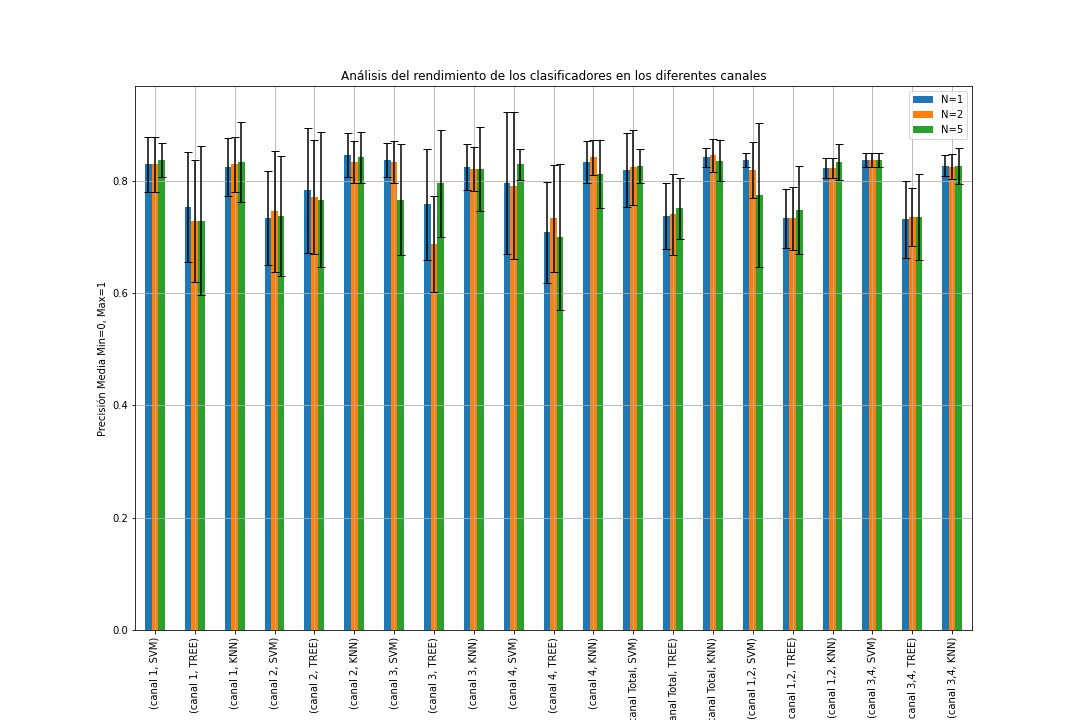
\includegraphics[width=1.0\textwidth]{imagenes/Grafica analisis final.jpg}
    \caption{Diagrama resumen de la precisión y desviación de cada clasificador}
    \label{fig:tabla resuemn}
\end{figure}

\newpage
Una vez vistas ambas tablas y la gráfica resumen de las precisiones podemos llegar a indagar en que clasificador es el más conveniente para nuestro problema. A continuación se muestra un breve resumen sobre los resultados obtenidos.
\subsubsection{Canal 1: vasto medial izquierdo}
La precisión más alta en este canal nos la da el SVM usando un archivo de entrenamiento-testeo con 5 características. 

\subsubsection{ Canal 2: recto femoral izquierdo}
En este canal la mejor precisión se obtiene con un KNN utilizando un número de vecinos de 6 y un archivo de entrenamiento-testeo con 1 característica. Su desviación típica es de las menores.

\subsubsection{Canal 3: vasto medial derecho}
En este canal la mejor precisión viene dada por un SVM con un archivo de entrenamiento-testeo con solo 1 característica. Además su desviación típica es bastante pequeña.

\subsubsection{Canal 4: recto femoral derecho}
En el canal 4 la mejor precisión nos la da un KNN utilizando un número de vecinos de 6 y un archivo de entrenamiento-testeo con 2 características.

\subsubsection{Canal 1,2: extremidad inferior izquierda}
Para el canal 1,2 el clasificador que nos da la mejor precisión es un SVM utilizando un archivo de entrenamiento-testeo con 1 característica.

\subsubsection{Canal 3,4: extremidad inferior derecha}
Para el canal 3,4 el clasificador que nos da la mejor precisión es un SVM utilizando tanto un archivo de entrenamiento-testeo con 1, 2 ó 5 características.

\subsubsection{Canal total: agrupación de todos los canales }
Para el canal total la mejor precisión viene dada por un KNN utilizando un número de vecinos de 6 y un archivo de entrenamiento-testeo con 2 características.




%4.2 Discusión
%Tras la presentación objetiva de los resultados, deberás aportar una discusión de los
%En este capítulo puedes discutir la relevancia de los resultados, presentar
%explicaciones para los resultados obtenidos (esperados o anómalos) y resaltar
%resultados que sean particularmente relevantes. Fíjate que a diferencia de la
%"Resultados", aquí se espera que incluyas tu opinión/reflexión sobre los resultados


\section{Discusión}
Como se ha ido explicando a lo largo del proyecto, la idea era desarrollar un clasificador para estimar la fatiga durante los entrenamientos y poder obtener conclusiones de anomalías en las rodillas de los pacientes y atletas. Además de esto, como ya se explicó en el capitulo \ref{tiposClasificadores}, se pretendía analizar diferentes situaciones debido a la ventaja de que la herramienta utilizada para tomar los datos llegaba a registrar los datos de 4 músculos diferentes. Por ello se optó por aumentar el estudio a diferentes niveles musculares.



\subsection{Modelos utilizados}
Los diferentes modelos que fueron utilizados para el proyecto han sido:
\begin{itemize}
\item Support vector machines (SVMs): máquinas de vector de soporte.
\item Decision trees (Trees): árboles de decisión.
\item K nearest neighbors (KNN): K vecinos más cercanos.
\end{itemize}

Viendo los resultados obtenidos (precisión y desviación) mediante la validación cruzada por cada uno de ellos, considero que el que mejor prestaciones ha dado ha sido el KNN con k = 6. Como se puede ver en la gráfica \ref{fig:tabla resuemn}, el clasificador KNN ha sido el que más estable se ha mantenido, dando en todas las situaciones estudiadas un rendimiento muy bueno y sin gran variación.

El hecho de que KNN obtenga una precisión mucho mayor a la de los árboles de decisión, pienso que se debe a que la fatiga muscular estudiada puede tener diferentes situaciones. Por ejemplo, que la fatiga esté representada en tres grupos diferentes. Estos tres grupos supongamos que tienen dichos valores:
\begin{itemize}
\item Grupo 1: RMS con valores altos, IEMG con valores bajos.
\item Grupo 2: RMS con valores bajos pero con un MNF con valores muy altos (cerca del 1).
\item Grupo 3: MAV con valores bajos y ZC con valores muy bajos (cerca del 0).
\end{itemize}

Esta situación daría 3 subgrupos representativos de la fatiga, por ello pienso que como el KNN divide todo el conjunto de datos en subgrupos, en este caso de k = 6 para determinar la nueva categoría, tiene mayor capacidad a la hora de determinar una categoría para una señal no conocida.


En segunda posición dejaría al SVM. Este clasificador también ha obtenido un buen rendimiento, pero en ciertas ocasiones una precisión muy baja y una gran variación indicada por los valores de su desviación, por lo que esto nos indica que hay veces en donde ha dado un rendimiento muy alto y otras ocasiones donde el rendimiento fue bajo. Se puede deber a que en ocasiones la fatiga no estaba realmente clara y su separación entre los vectores de soporte era muy pequeña y debido a esto el clasificador no era capaz de clasificar algunos datos correctamente.

En tercera y última posición situaría al Desion Tree. Pienso que ha sido el que peores resultados ha obtenido. En todas las situaciones estudiadas ha dado la precisión mas baja y con una gran variación.

Los árboles de decisión van realizando ramificaciones para determinar la categoría final de los datos de testeo y esto puede hacer que como no hay un patrón realmente claro en la fatiga con las características utilizadas, que no se obtenga un rendimiento del todo estable. Otra posibilidad de este rendimiento, se debe a que el conjunto de datos utilizados consta de un número mucho mayor de no fatiga = 0, que de fatiga = 1. Por ello, el árbol de decisión puede sesgar los datos al haber una clase dominante.

En conclusión, yo personalmente me quedaría con un clasificador SVM o KNN. A continuación se hace una valoración del rendimiento de cada uno de estos en los diferentes canales estudiados.

\subsection{Canal 1, canal 2, canal 3, canal 4}
Los datos obtenidos son bastantes curiosos. Podemos ver que para tanto el canal 1 como para el canal 3 (ambos registraban información del vasto medial, solo que uno de la pierna derecha y otro de la pierna izquierda) la mejor opción es el SVM.

Sin embargo, tanto para el canal 2 como para el canal 4 (ambos registraban información del recto femoral , uno en la pierna derecha y otro en la izquierda) la mejor opción es un KNN. 


Esto podría justificarse, ya que la sentadilla es un ejercicio muy demandante de vasto medial. Como se puede ver en este estudio \cite{muyor2020actividad}, donde se analiza que músculos del cuadriceps realizan una mayor activación a la hora de realizar diferentes sentadillas. Es decir, aunque el recto femoral también forma parte del cuadricpes y apoya el movimiento de la rodilla junto con el vasto medial, es el vasto medial el músculo más implicado.

Debido a esto, la señal de los canales del vasto medial puede llegar a ser más intensa que la de los canales del recto femoral. Esto puede hacer que la fatiga quede mejor definida en estos casos, ya que al tener una mayor activación, es lógico que dicho músculo se fatigue antes. Por ello pienso que los dos grupos definidos en el SVM pueden quedar definidos con una mayor separación entre los dos vectores de soporte de cada grupo y por ello clasificar mejor los datos no conocidos.

Otro factor a tener en cuenta es que la desviación típica del clasificador SVM en los respectivos canales del recto femoral, es muy alta. Puede ser debido a que como la señal no tiene valores tan característicos de la fatiga, haya veces donde los dos grupos definidos por los vectores de soporte correspondientes queden mejor definidos y otras veces peor definidos.


Por otro lado el clasificador KNN, al determinar la nueva categoría basándose en sus k vecinos más cercanos, puede llegar a clasificar mejor los datos que estén menos "definidos", es decir, menos representativos de la fatiga en ese caso.

En resumen, pienso que el clasificador SVM puede llegar a tener mejores prestaciones con datos musculares de músculos más demandantes, mientras que el KNN puede ser mejor para analizar la señal muscular en músculos menos demandantes.

\subsection{Canal 1,2 y canal 3,4}
Otra de la observación  que se puede hacer, y relacionada con la conclusión anterior, es que una vez que se utiliza un clasificador para detectar la fatiga global de la extremidad inferior, ya sea derecha o izquierda, el clasificador que mejor prestaciones nos da es el SVM. 

Esto se puede dar debido a que el canal 1,2 trata de la agrupación de los datos captados por el electromiógrafo en el canal 1 y en el canal 2. Como individualmente para estos dos canales separados, el SVM obtenía mejores prestaciones en el canal del vasto medial y este era el más demandante, para la agrupación de los datos en el canal 1,2 también lo será. Cabe destacar que esto también se cumple en el canal 3,4.

Como se explicó en la sección anterior, como el vasto medial tiene mayor activación, esto puede hacer que a la hora de clasificar los datos agrupados en canales de una misma extremidad, sea el vasto medial el más representativo de la fatiga y por ende el clasificador SVM el que mejor prestaciones nos da, ya que conseguiría dos grupos mejor definidos.

\subsection{Canal total: agrupación de todos los canales}
Sin embargo, para el clasificador de la fatiga global, el mejor rendimiento viene dado por un KNN utilizando un número de vecinos de 6 y dos características en el archivo de entrenamiento-testeo.

Mi opinión es que a la hora de juntar todos los canales en un canal total, es decir, agrupar los datos recibidos de los 4 canales, el conjunto de datos se hace muy grande. Esto hace que el SVM decaiga en prestaciones, ya que no podrá definir un modelo con dos grupos claramente diferenciados.

Debido a esto el KNN obtiene mejores prestaciones, ya que como se explicó anteriormente, basa su predicción en sus k vecinos y esto dota al modelo de una mayor flexibilidad a la hora de predecir la fatiga.

\subsection{Número de características en los archivos de \newline entrenamiento-testeo}
Aunque hay veces que la mayor precisión se obtiene solo con una característica en el archivo de entrenamiento-testeo, existe un gran número de ocasiones donde el mejor rendimiento viene dado por 2 o incluso 5 características. Esto se puede dar debido a que la fatiga es compleja de clasificar solo teniendo en cuenta las características de la señal.

Pueden existir ocasiones donde con sola una característica no sea capaz de clasificar bien la fatiga. Este aumento de las características utilizadas aunque nos daría un modelo mas complejo, sería complementado con un aumento de la precisión de nuestro modelo.


\subsection{Mejor opción para el proyecto}
Después de realizar el análisis de los resultados obtenidos, me decantaría por la opción de utilizar un clasificador por grupo muscular estudiado. Esto es, la opción de los clasificadores del canal 1, canal 2, canal 3 y canal 4, donde para los canales 1 y 3, utilizaría un SVM y para los canales 2 y 4 un KNN.

Pienso que es la opción que mejor rendimiento aporta a la resolución de nuestro problema, ya que nos da un nivel de exactitud muy alto a la hora de analizar 4 músculos diferentes y con ello, se podrá analizar cuál de los 4 entra antes en fatiga y llegar a conclusiones más especificas, como compensación muscular, anomalías en la rodilla o falta de capacidad muscular.


\subsection{Limitaciones}
Sobre las limitaciones del proyecto, me gustaría destacar que hay ocasiones donde la mejor opción es un clasificador KNN. Como se vio en la fase de diseño, este clasificador utiliza un K = 6, es decir, el número de vecinos para determinar la nueva etiqueta es 6. 

Debido a esto, si finalmente a la hora de llevar el proyecto al mercado o simplemente como complemento a la aplicación de mDurance, se elige la opción del KNN, sería conveniente realizar un estudio para estimar cual sería el K, que mejor prestaciones nos da.


También pienso que sería correcto probar los clasificadores estudiados con un conjunto de datos más grande. Para este proyecto se han utilizado 19 muestras y cada muestra contenía 4 señales de EMG. Con un conjunto de datos más grandes, quizá se podrían obtener unas conclusiones con una mayor validez.

%aqui resultados y discusión
%
\chapter{Conclusiones y Trabajos Futuros}
Este capítulo está dedicado a realizar una conclusión final sobre el proyecto y a analizar si realmente se han cumplido los objetivos que se tenían antes de su comienzo. (Objetivos \ref{objetivos}).

\section{Conclusiones}

El objetivo final de este proyecto era el de diseñar un clasificador para detectar la fatiga muscular y así poder detectar anomalías en la rodilla. Pienso que este objetivo se ha cumplido satisfactoriamente ya que se ha realizado un análisis sobre el rendimiento de diversos clasificadores que resolvían el problema. Con ello se ha obtenido el clasificador con las mejores prestaciones. 

Con respecto a los objetivos específicos, se ha conseguido analizar y procesar las señales brutas de EMG. Esto se ha resuelto con el hecho de detectar la activación muscular de cada repetición registrada para así estimar el tamaño de ventana correcto.

Otro de los objetivos específicos fue analizar las velocidades registradas para estimar la fatiga de cada repetición. Para ello se acordó la estimación de un umbral de fatiga y la condición de que dicho umbral tenia que registrase dos veces seguidas.

El siguiente objetivo específico y uno de los más importantes fue la extracción de características. Este objetivo es primordial ya que nos dota de la información necesaria para poder clasificar en un futuro las señales. Opino que se ha cumplido correctamente, ya que se han estudiado 15 características diferentes de la señal EMG.

El objetivo de la creación de los archivos de entrenamiento-testeo también creo que se ha cumplido correctamente. Se han analizado los clasificadores con diferentes archivos de entrenamiento-testeo obtenidos gracias al procesamiento y extracción de las características de la señal EMG, tanto en el dominio del tiempo como en el dominio de la frecuencia.

Otro de los objetivos importantes, era el diseño de un algoritmo de selección de características, para obtener unos modelos sencillos y eficaces. Para ello se ha indagado en el tema de la selección de características y llegado a la conclusión de que uno de los mejores algoritmos para ello era el RFE (Recursive Feautre Elimination).

Los dos últimos objetivos, también se han realizado correctamente. Uno de ellos era investigar sobre que tipo de clasificadores de aprendizaje supervisado era el más adecuado para la resolución del proyecto. 

El último objetivo, que es complementario al anterior, ha sido la validación de los resultados obtenidos por los clasificadores. Para ello se ha hecho uso de la validación cruzada, para estimar así una precisión y desviación a cada clasificador en cada una de las situaciones estudiadas.


Como conclusión final, lo que se ha conseguido es realizar un estudio sobre que clasificador sería el mejor a la hora de resolver el problema de la detección de la fatiga. Además se ha indagado en el problema, y también se aportan diferentes soluciones, en caso de que la herramienta futura que se utilice no disponga de 4 canales de registro de la actividad muscular. 


Mi opinión es que se ha realizado un proyecto muy interesante, donde era necesario indagar e investigar en cada uno de los objetivos específicos para llegar a obtener una buena solución para el objetivo general del proyecto.



\section{Trabajos Futuros}
Con respecto a los trabajos futuros creo que es un proyecto muy interesante que aporta una gran cantidad de información sobre que tipos de clasificadores y condiciones son las óptimas si se quiere llevar al mercado esta idea.

Debido a todo lo comentado anteriormente, pienso que se ha realizado un buen proyecto, que puede ser utilizado por algún emprendedor, como recurso para ver que sistema de clasificación sería mas conveniente implementar y desarrollar en un sistema de EMG final, para llevarlo al mercado y que sea utilizado por los médicos y fisioterapeutas. Por ejemplo, sería de gran utilidad que si un paciente siente molestia en su rodilla durante la actividad física o su vida cotidiana, realizar un análisis con una herramienta como la explicada en este proyecto y analizar el rendimiento de la musculatura de su pierna.

También podría ser un complemento a la herramienta base de mDurance. Dicha herramienta solo capta, analiza la señal EMG y extrae las correspondientes características. Con este nuevo complemento, también se dotaría al fisioterapeuta de una opción para analizar la fatiga muscular. Se podría hallar que músculos se han fatigado antes, y si se ha producido dicha fatiga, el orden en que se han fatigado, ya que una alteración en la fatiga puede ser indicativo de una compensación muscular debido a una lesión. (Para mayor detalle ver \ref{compM}).

Para finalizar cabe aclarar que esta herramienta, es claramente orientativa para médicos y fisioterapeutas. Serviría de apoyo a la hora de realizar sus diagnósticos. Ellos son los que realmente tienen la última palabra sobre el diagnostico.



%
%%\chapter{Conclusiones y Trabajos Futuros}
\nocite{*}
\bibliographystyle{plain}
\bibliography{bibliografia/bibliografia}
\addcontentsline{toc}{chapter}{Bibliografía}
\bibliographystyle{miunsrturl}

%
\appendix
\input{apendices/Anexo}
%\input{apendices/manual_usuario/manual_usuario}
%%\input{apendices/paper/paper}
%\input{glosario/entradas_glosario}
% \addcontentsline{toc}{chapter}{Glosario}
% \printglossary
\chapter*{}
\thispagestyle{empty}

\end{document}
